\newpage
\appendix
\section{Appendix} \label{appendix}
%
%%\begin{figure}[h]
%%	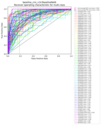
\includegraphics[width=0.8\textwidth]{bilder/ROC-multiclass.png}
%%	\caption{Example for a ROC-Curve obtained during evaluation. The numbers in the legend are the \textit{SNOMED} codes for the classes. Micro and Macro are the averages along the classes.}
%%	\label{fig:roc-example}
%%	\centering
%%\end{figure}
%
%\subsection{Baseline Results}
%\begin{figure}
%	\captionof{table}{Baseline F1 scores}
%	\begin{subfigure}[b]{0.49\hsize}\centering
%		\input{"/home/julian/Downloads/Github/contrastive-predictive-coding/models/25_06_21-16-test|bl_FCN+bl_MLP+bl_TCN_block+bl_TCN_down+bl_TCN_flatten+bl_TCN_last+bl_alex_v2+bl_cnn_v0+bl_cnn_v0_1+bl_cnn_v0_2+bl_cnn_v0_3+bl_cnn_v1+bl_cnn_v14+bl_cnn_v15+bl_cnn_v2+bl_cnn_v3+bl_cnn_v4+bl_cnn_v5+bl_cnn_v6+bl_cnn_v7+bl_cnn_v8+bl_cnn_v9+/f1-scores-avg-dataloader0.tex"}
%		\caption{Models trained with class weights in the loss function.}
%		\label{tbl:f1scores-avg-bl-class}	
%	\end{subfigure}%
%	\begin{subfigure}[b]{0.49\hsize}\centering
%		\input{"/home/julian/Downloads/Github/contrastive-predictive-coding/models/26_06_21-15-test|(2x)bl_MLP+bl_FCN+bl_TCN_block+bl_TCN_down+bl_TCN_flatten+bl_TCN_last+bl_alex_v2+bl_cnn_v0+bl_cnn_v0_1+bl_cnn_v0_2+bl_cnn_v0_3+bl_cnn_v1+bl_cnn_v14+bl_cnn_v15+bl_cnn_v2+bl_cnn_v3+bl_cnn_v4+bl_cnn_v5+bl_cnn_v6+bl_cnn_v7+bl_cnn_v8+bl_cnn/f1-scores-avg-dataloader0.tex"}
%		\caption{Models trained without class weights in the loss function.}	
%		\label{tbl:f1scores-avg-bl-noclass}
%	\end{subfigure}
%\end{figure}
%\begin{figure}
%	\captionof{table}{Baseline Precision scores}
%	\begin{subfigure}[b]{0.49\hsize}\centering
%		\input{/home/julian/Downloads/Github/contrastive-predictive-coding/models/25_06_21-16-test|bl_FCN+bl_MLP+bl_TCN_block+bl_TCN_down+bl_TCN_flatten+bl_TCN_last+bl_alex_v2+bl_cnn_v0+bl_cnn_v0_1+bl_cnn_v0_2+bl_cnn_v0_3+bl_cnn_v1+bl_cnn_v14+bl_cnn_v15+bl_cnn_v2+bl_cnn_v3+bl_cnn_v4+bl_cnn_v5+bl_cnn_v6+bl_cnn_v7+bl_cnn_v8+bl_cnn_v9+/precision-scores-avg-dataloader0.tex}
%		\caption{Models trained with class weights in the loss function.}
%		\label{tbl:precscores-avg-bl-class}	
%	\end{subfigure}%
%	\vline
%	\begin{subfigure}[b]{0.49\hsize}\centering
%		\input{/home/julian/Downloads/Github/contrastive-predictive-coding/models/26_06_21-15-test|(2x)bl_MLP+bl_FCN+bl_TCN_block+bl_TCN_down+bl_TCN_flatten+bl_TCN_last+bl_alex_v2+bl_cnn_v0+bl_cnn_v0_1+bl_cnn_v0_2+bl_cnn_v0_3+bl_cnn_v1+bl_cnn_v14+bl_cnn_v15+bl_cnn_v2+bl_cnn_v3+bl_cnn_v4+bl_cnn_v5+bl_cnn_v6+bl_cnn_v7+bl_cnn_v8+bl_cnn/precision-scores-avg-dataloader0.tex}
%		\caption{Models trained without class weights in the loss function.}	
%		\label{tbl:precscores-avg-bl-noclass}
%	\end{subfigure}
%\end{figure}
%\begin{figure}
%	\captionof{table}{Baseline Recall scores}
%	\begin{subfigure}[b]{0.49\hsize}\centering
%		\input{/home/julian/Downloads/Github/contrastive-predictive-coding/models/25_06_21-16-test|bl_FCN+bl_MLP+bl_TCN_block+bl_TCN_down+bl_TCN_flatten+bl_TCN_last+bl_alex_v2+bl_cnn_v0+bl_cnn_v0_1+bl_cnn_v0_2+bl_cnn_v0_3+bl_cnn_v1+bl_cnn_v14+bl_cnn_v15+bl_cnn_v2+bl_cnn_v3+bl_cnn_v4+bl_cnn_v5+bl_cnn_v6+bl_cnn_v7+bl_cnn_v8+bl_cnn_v9+/recall-scores-avg-dataloader0.tex}
%		\caption{Models trained with class weights in the loss function.}
%		\label{tbl:recscores-avg-bl-class}	
%	\end{subfigure}%
%	\begin{subfigure}[b]{0.49\hsize}\centering
%		\input{/home/julian/Downloads/Github/contrastive-predictive-coding/models/26_06_21-15-test|(2x)bl_MLP+bl_FCN+bl_TCN_block+bl_TCN_down+bl_TCN_flatten+bl_TCN_last+bl_alex_v2+bl_cnn_v0+bl_cnn_v0_1+bl_cnn_v0_2+bl_cnn_v0_3+bl_cnn_v1+bl_cnn_v14+bl_cnn_v15+bl_cnn_v2+bl_cnn_v3+bl_cnn_v4+bl_cnn_v5+bl_cnn_v6+bl_cnn_v7+bl_cnn_v8+bl_cnn/recall-scores-avg-dataloader0.tex}
%		\caption{Models trained without class weights in the loss function.}	
%		\label{tbl:recscores-avg-bl-noclass}
%	\end{subfigure}
%\end{figure}
%\begin{figure}
%	\captionof{table}{Baseline Custom Accuracy (Class Fit) scores}
%	\begin{subfigure}[b]{0.49\hsize}\centering
%		\input{/home/julian/Downloads/Github/contrastive-predictive-coding/models/25_06_21-16-test|bl_FCN+bl_MLP+bl_TCN_block+bl_TCN_down+bl_TCN_flatten+bl_TCN_last+bl_alex_v2+bl_cnn_v0+bl_cnn_v0_1+bl_cnn_v0_2+bl_cnn_v0_3+bl_cnn_v1+bl_cnn_v14+bl_cnn_v15+bl_cnn_v2+bl_cnn_v3+bl_cnn_v4+bl_cnn_v5+bl_cnn_v6+bl_cnn_v7+bl_cnn_v8+bl_cnn_v9+/Custom Accuracy (Class Fit)scores-avg-dataloader-0.tex}
%		\caption{Models trained with class weights in the loss function.}
%		\label{tbl:recscores-avg-bl-class}	
%	\end{subfigure}%
%	\begin{subfigure}[b]{0.49\hsize}\centering
%		\input{/home/julian/Downloads/Github/contrastive-predictive-coding/models/26_06_21-15-test|(2x)bl_MLP+bl_FCN+bl_TCN_block+bl_TCN_down+bl_TCN_flatten+bl_TCN_last+bl_alex_v2+bl_cnn_v0+bl_cnn_v0_1+bl_cnn_v0_2+bl_cnn_v0_3+bl_cnn_v1+bl_cnn_v14+bl_cnn_v15+bl_cnn_v2+bl_cnn_v3+bl_cnn_v4+bl_cnn_v5+bl_cnn_v6+bl_cnn_v7+bl_cnn_v8+bl_cnn/Custom Accuracy (Class Fit)scores-avg-dataloader-0.tex}
%		\caption{Models trained without class weights in the loss function.}	
%		\label{tbl:recscores-avg-bl-noclass}
%	\end{subfigure}
%\end{figure}
%\begin{figure}
%	\captionof{table}{Baseline Custom Accuracy (Zero Fit) scores}
%	\begin{subfigure}[b]{0.49\hsize}\centering
%		\input{/home/julian/Downloads/Github/contrastive-predictive-coding/models/25_06_21-16-test|bl_FCN+bl_MLP+bl_TCN_block+bl_TCN_down+bl_TCN_flatten+bl_TCN_last+bl_alex_v2+bl_cnn_v0+bl_cnn_v0_1+bl_cnn_v0_2+bl_cnn_v0_3+bl_cnn_v1+bl_cnn_v14+bl_cnn_v15+bl_cnn_v2+bl_cnn_v3+bl_cnn_v4+bl_cnn_v5+bl_cnn_v6+bl_cnn_v7+bl_cnn_v8+bl_cnn_v9+/Custom Accuracy (Zero Fit)scores-avg-dataloader-0.tex}
%		\caption{Models trained with class weights in the loss function.}
%		\label{tbl:recscores-avg-bl-class}	
%	\end{subfigure}%
%	\begin{subfigure}[b]{0.49\hsize}\centering
%		\input{/home/julian/Downloads/Github/contrastive-predictive-coding/models/26_06_21-15-test|(2x)bl_MLP+bl_FCN+bl_TCN_block+bl_TCN_down+bl_TCN_flatten+bl_TCN_last+bl_alex_v2+bl_cnn_v0+bl_cnn_v0_1+bl_cnn_v0_2+bl_cnn_v0_3+bl_cnn_v1+bl_cnn_v14+bl_cnn_v15+bl_cnn_v2+bl_cnn_v3+bl_cnn_v4+bl_cnn_v5+bl_cnn_v6+bl_cnn_v7+bl_cnn_v8+bl_cnn/Custom Accuracy (Zero Fit)scores-avg-dataloader-0.tex}
%		\caption{Models trained without class weights in the loss function.}	
%		\label{tbl:recscores-avg-bl-noclass}
%	\end{subfigure}
%\end{figure}
%
%\subsection{CPC Results}
%\begin{figure}
%	\captionof{table}{CPC F1 scores}
%	\begin{subfigure}[b]{0.49\hsize}\centering
%		\input{"/home/julian/Downloads/Github/contrastive-predictive-coding/models/09_07_21-17-test|(34x)cpc/f1-scores-avg-dataloader0.tex"}
%		\caption{Models trained with class weights in the loss function.}
%		\label{tbl:f1scores-avg-cpc-class}	
%	\end{subfigure}%
%	\begin{subfigure}[b]{0.49\hsize}\centering
%		\input{"/home/julian/Downloads/Github/contrastive-predictive-coding/models/16_06_21-15-test|(2x)bl_FCN+(2x)bl_cnn_v0+(2x)bl_cnn_v0_1+(2x)bl_cnn_v0_2+(2x)bl_cnn_v0_3+(2x)bl_cnn_v1+(2x)bl_cnn_v14+(2x)bl_cnn_v2+(2x)bl_cnn_v3+(2x)bl_cnn_v4+(2x)bl_cnn_v5+(2x)bl_cnn_v6+(2x)bl_cnn_v8+(2x)bl_cnn_v9+(50x)cpc+bl_MLP/CPC|no-class-weights/f1-scores-avg-dataloader0.tex"}
%		\caption{Models trained without class weights in the loss function.}	
%		\label{tbl:f1scores-avg-cpc-noclass}
%	\end{subfigure}
%\end{figure}
%\begin{figure}
%	\captionof{table}{CPC Precision scores}
%	\begin{subfigure}[b]{0.49\hsize}\centering
%		\input{/home/julian/Downloads/Github/contrastive-predictive-coding/models/09_07_21-17-test|(34x)cpc/precision-scores-avg-dataloader0.tex}
%		\caption{Models trained with class weights in the loss function.}
%		\label{tbl:precscores-avg-cpc-class}	
%	\end{subfigure}%
%	\vline
%	\begin{subfigure}[b]{0.49\hsize}\centering
%		\input{/home/julian/Downloads/Github/contrastive-predictive-coding/models/16_06_21-15-test|(2x)bl_FCN+(2x)bl_cnn_v0+(2x)bl_cnn_v0_1+(2x)bl_cnn_v0_2+(2x)bl_cnn_v0_3+(2x)bl_cnn_v1+(2x)bl_cnn_v14+(2x)bl_cnn_v2+(2x)bl_cnn_v3+(2x)bl_cnn_v4+(2x)bl_cnn_v5+(2x)bl_cnn_v6+(2x)bl_cnn_v8+(2x)bl_cnn_v9+(50x)cpc+bl_MLP/CPC|no-class-weights/precision-scores-avg-dataloader0.tex}
%		\caption{Models trained without class weights in the loss function.}	
%		\label{tbl:precscores-avg-cpc-noclass}
%	\end{subfigure}
%\end{figure}
%\begin{figure}
%	\captionof{table}{CPC Recall scores}
%	\begin{subfigure}[b]{0.49\hsize}\centering
%		\input{/home/julian/Downloads/Github/contrastive-predictive-coding/models/09_07_21-17-test|(34x)cpc/recall-scores-avg-dataloader0.tex}
%		\caption{Models trained with class weights in the loss function.}
%		\label{tbl:recscores-avg-cpc-class}	
%	\end{subfigure}%
%	\begin{subfigure}[b]{0.49\hsize}\centering
%		\input{/home/julian/Downloads/Github/contrastive-predictive-coding/models/16_06_21-15-test|(2x)bl_FCN+(2x)bl_cnn_v0+(2x)bl_cnn_v0_1+(2x)bl_cnn_v0_2+(2x)bl_cnn_v0_3+(2x)bl_cnn_v1+(2x)bl_cnn_v14+(2x)bl_cnn_v2+(2x)bl_cnn_v3+(2x)bl_cnn_v4+(2x)bl_cnn_v5+(2x)bl_cnn_v6+(2x)bl_cnn_v8+(2x)bl_cnn_v9+(50x)cpc+bl_MLP/CPC|no-class-weights/recall-scores-avg-dataloader0.tex}
%		\caption{Models trained without class weights in the loss function.}	
%		\label{tbl:recscores-avg-cpc-noclass}
%	\end{subfigure}
%\end{figure}
%\begin{figure}
%	\captionof{table}{CPC Custom Accuracy (Class Fit) scores}
%	\begin{subfigure}[b]{0.49\hsize}\centering
%		\input{/home/julian/Downloads/Github/contrastive-predictive-coding/models/09_07_21-17-test|(34x)cpc/Custom Accuracy (Class Fit)scores-avg-dataloader-0.tex}
%		\caption{Models trained with class weights in the loss function.}
%		\label{tbl:recscores-avg-cpc-class}	
%	\end{subfigure}%
%	\begin{subfigure}[b]{0.49\hsize}\centering
%		\input{/home/julian/Downloads/Github/contrastive-predictive-coding/models/16_06_21-15-test|(2x)bl_FCN+(2x)bl_cnn_v0+(2x)bl_cnn_v0_1+(2x)bl_cnn_v0_2+(2x)bl_cnn_v0_3+(2x)bl_cnn_v1+(2x)bl_cnn_v14+(2x)bl_cnn_v2+(2x)bl_cnn_v3+(2x)bl_cnn_v4+(2x)bl_cnn_v5+(2x)bl_cnn_v6+(2x)bl_cnn_v8+(2x)bl_cnn_v9+(50x)cpc+bl_MLP/CPC|no-class-weights/Custom Accuracy (Class Fit)scores-avg-dataloader-0.tex}
%		\caption{Models trained without class weights in the loss function.}	
%		\label{tbl:recscores-avg-cpc-noclass}
%	\end{subfigure}
%\end{figure}
%\begin{figure}
%	\captionof{table}{CPC Custom Accuracy (Zero Fit) scores}
%	\begin{subfigure}[b]{0.49\hsize}\centering
%		\input{/home/julian/Downloads/Github/contrastive-predictive-coding/models/09_07_21-17-test|(34x)cpc/Custom Accuracy (Zero Fit)scores-avg-dataloader-0.tex}
%		\caption{Models trained with class weights in the loss function.}
%		\label{tbl:recscores-avg-cpc-class}	
%	\end{subfigure}%
%	\begin{subfigure}[b]{0.49\hsize}\centering
%		\input{/home/julian/Downloads/Github/contrastive-predictive-coding/models/16_06_21-15-test|(2x)bl_FCN+(2x)bl_cnn_v0+(2x)bl_cnn_v0_1+(2x)bl_cnn_v0_2+(2x)bl_cnn_v0_3+(2x)bl_cnn_v1+(2x)bl_cnn_v14+(2x)bl_cnn_v2+(2x)bl_cnn_v3+(2x)bl_cnn_v4+(2x)bl_cnn_v5+(2x)bl_cnn_v6+(2x)bl_cnn_v8+(2x)bl_cnn_v9+(50x)cpc+bl_MLP/CPC|no-class-weights/Custom Accuracy (Zero Fit)scores-avg-dataloader-0.tex}
%		\caption{Models trained without class weights in the loss function.}	
%		\label{tbl:recscores-avg-cpc-noclass}
%	\end{subfigure}
%\end{figure}
%
%
%
%%\begin{minipage}[b]{1\hsize}\centering
%%	
%%	\captionof{table}{CPC F1 scores with class\_weights}
%%	\label{tbl:f1scores-avg-cpc-class}
%%	\input{"/home/julian/Downloads/Github/contrastive-predictive-coding/models/16_06_21-15-test|(2x)bl_FCN+(2x)bl_cnn_v0+(2x)bl_cnn_v0_1+(2x)bl_cnn_v0_2+(2x)bl_cnn_v0_3+(2x)bl_cnn_v1+(2x)bl_cnn_v14+(2x)bl_cnn_v2+(2x)bl_cnn_v3+(2x)bl_cnn_v4+(2x)bl_cnn_v5+(2x)bl_cnn_v6+(2x)bl_cnn_v8+(2x)bl_cnn_v9+(50x)cpc+bl_MLP/CPC|class-weights/f1-scores-avg-dataloader0.tex"}
%%	\captionof{table}{Models trained with class weights in the loss function. Legend:\newline
%%		\hl{m:all} All latents are used as negative examples in the cpc loss.
%%		\hl{m:same} Latents only from the same timestep are used as negative examples.
%%		\hl{linear/cnn/twolinear/latent\_maximum} the used downstream architecture.
%%		\hl{dte:x} Trained for x downstream epochs.
%%		\hl{pte:x} Trained for x pretrain epochs}
%%\end{minipage}
%%\begin{minipage}[b]{1\hsize}\centering
%%	\captionof{table}{CPC F1 scores without class\_weights}
%%	\label{tbl:f1scores-avg-cpc-noclass}
%%	\input{"/home/julian/Downloads/Github/contrastive-predictive-coding/models/16_06_21-15-test|(2x)bl_FCN+(2x)bl_cnn_v0+(2x)bl_cnn_v0_1+(2x)bl_cnn_v0_2+(2x)bl_cnn_v0_3+(2x)bl_cnn_v1+(2x)bl_cnn_v14+(2x)bl_cnn_v2+(2x)bl_cnn_v3+(2x)bl_cnn_v4+(2x)bl_cnn_v5+(2x)bl_cnn_v6+(2x)bl_cnn_v8+(2x)bl_cnn_v9+(50x)cpc+bl_MLP/CPC|no-class-weights/f1-scores-avg-dataloader0.tex"}
%%	\captionof{table}{Models trained with class weights in the loss function. Legend:\newline
%%		frozen}	
%%\end{minipage}
%%
%%\begin{minipage}[b]{0.49\hsize}\centering
%%	\captionof{table}{Baseline precision scores with class\_weights}
%%	\label{tbl:precisionscores-avg-bl-class}
%%	\input{"/home/julian/Downloads/Github/contrastive-predictive-coding/models/16_06_21-15-test|(2x)bl_FCN+(2x)bl_cnn_v0+(2x)bl_cnn_v0_1+(2x)bl_cnn_v0_2+(2x)bl_cnn_v0_3+(2x)bl_cnn_v1+(2x)bl_cnn_v14+(2x)bl_cnn_v2+(2x)bl_cnn_v3+(2x)bl_cnn_v4+(2x)bl_cnn_v5+(2x)bl_cnn_v6+(2x)bl_cnn_v8+(2x)bl_cnn_v9+(50x)cpc+bl_MLP/BL|class-weights/precision-scores-avg-dataloader0.tex"}
%%	\captionof{table}{Models trained with class weights in the loss function.}	
%%\end{minipage}%
%%\begin{minipage}[b]{0.49\hsize}\centering
%%	\captionof{table}{Baseline precision scores without class\_weights}
%%	\label{tbl:precisionscores-avg-bl-noclass}
%%	\input{"/home/julian/Downloads/Github/contrastive-predictive-coding/models/16_06_21-15-test|(2x)bl_FCN+(2x)bl_cnn_v0+(2x)bl_cnn_v0_1+(2x)bl_cnn_v0_2+(2x)bl_cnn_v0_3+(2x)bl_cnn_v1+(2x)bl_cnn_v14+(2x)bl_cnn_v2+(2x)bl_cnn_v3+(2x)bl_cnn_v4+(2x)bl_cnn_v5+(2x)bl_cnn_v6+(2x)bl_cnn_v8+(2x)bl_cnn_v9+(50x)cpc+bl_MLP/BL|no-class-weights/precision-scores-avg-dataloader0.tex"}
%%	\captionof{table}{Models trained without class weights in the loss function.}	
%%\end{minipage}
%%
%%\begin{minipage}[b]{1\hsize}\centering
%%	
%%	\captionof{table}{CPC precision scores with class\_weights}
%%	\label{tbl:precisionscores-avg-cpc-class}
%%	\input{"/home/julian/Downloads/Github/contrastive-predictive-coding/models/16_06_21-15-test|(2x)bl_FCN+(2x)bl_cnn_v0+(2x)bl_cnn_v0_1+(2x)bl_cnn_v0_2+(2x)bl_cnn_v0_3+(2x)bl_cnn_v1+(2x)bl_cnn_v14+(2x)bl_cnn_v2+(2x)bl_cnn_v3+(2x)bl_cnn_v4+(2x)bl_cnn_v5+(2x)bl_cnn_v6+(2x)bl_cnn_v8+(2x)bl_cnn_v9+(50x)cpc+bl_MLP/CPC|class-weights/precision-scores-avg-dataloader0.tex"}
%%	\captionof{table}{Models trained with class weights in the loss function. Legend:\newline
%%		\hl{m:all} All latents are used as negative examples in the cpc loss.
%%		\hl{m:same} Latents only from the same timestep are used as negative examples.
%%		\hl{linear/cnn/twolinear/latent\_maximum} the used downstream architecture.
%%		\hl{dte:x} Trained for x downstream epochs.
%%		\hl{pte:x} Trained for x pretrain epochs}
%%\end{minipage}
%%\begin{minipage}[b]{1\hsize}\centering
%%	\captionof{table}{CPC precision scores without class\_weights}
%%	\label{tbl:precisionscores-avg-cpc-noclass}
%%	\input{"/home/julian/Downloads/Github/contrastive-predictive-coding/models/16_06_21-15-test|(2x)bl_FCN+(2x)bl_cnn_v0+(2x)bl_cnn_v0_1+(2x)bl_cnn_v0_2+(2x)bl_cnn_v0_3+(2x)bl_cnn_v1+(2x)bl_cnn_v14+(2x)bl_cnn_v2+(2x)bl_cnn_v3+(2x)bl_cnn_v4+(2x)bl_cnn_v5+(2x)bl_cnn_v6+(2x)bl_cnn_v8+(2x)bl_cnn_v9+(50x)cpc+bl_MLP/CPC|no-class-weights/precision-scores-avg-dataloader0.tex"}
%%	\captionof{table}{Models trained with class weights in the loss function. Legend:\newline
%%		frozen}	
%%\end{minipage}
%%
%%\begin{minipage}[b]{0.49\hsize}\centering
%%	\captionof{table}{Baseline Custom Accuracy (Class Fit) scores with class\_weights}
%%	\label{tbl:Custom Accuracy (Class Fit)scores-avg-bl-class}
%%	\input{"/home/julian/Downloads/Github/contrastive-predictive-coding/models/16_06_21-15-test|(2x)bl_FCN+(2x)bl_cnn_v0+(2x)bl_cnn_v0_1+(2x)bl_cnn_v0_2+(2x)bl_cnn_v0_3+(2x)bl_cnn_v1+(2x)bl_cnn_v14+(2x)bl_cnn_v2+(2x)bl_cnn_v3+(2x)bl_cnn_v4+(2x)bl_cnn_v5+(2x)bl_cnn_v6+(2x)bl_cnn_v8+(2x)bl_cnn_v9+(50x)cpc+bl_MLP/BL|class-weights/Custom Accuracy (Class Fit)scores-avg-dataloader-0.tex"}
%%	\captionof{table}{Models trained with class weights in the loss function.}	
%%\end{minipage}%
%%\begin{minipage}[b]{0.49\hsize}\centering
%%	\captionof{table}{Baseline Custom Accuracy (Class Fit) scores without class\_weights}
%%	\label{tbl:Custom Accuracy (Class Fit)scores-avg-bl-noclass}
%%	\input{"/home/julian/Downloads/Github/contrastive-predictive-coding/models/16_06_21-15-test|(2x)bl_FCN+(2x)bl_cnn_v0+(2x)bl_cnn_v0_1+(2x)bl_cnn_v0_2+(2x)bl_cnn_v0_3+(2x)bl_cnn_v1+(2x)bl_cnn_v14+(2x)bl_cnn_v2+(2x)bl_cnn_v3+(2x)bl_cnn_v4+(2x)bl_cnn_v5+(2x)bl_cnn_v6+(2x)bl_cnn_v8+(2x)bl_cnn_v9+(50x)cpc+bl_MLP/BL|no-class-weights/Custom Accuracy (Class Fit)scores-avg-dataloader-0.tex"}
%%	\captionof{table}{Models trained without class weights in the loss function.}	
%%\end{minipage}
%%
%%\begin{minipage}[b]{1\hsize}\centering
%%	
%%	\captionof{table}{CPC Custom Accuracy (Class Fit) scores with class\_weights}
%%	\label{tbl:Custom Accuracy (Class Fit)scores-avg-cpc-class}
%%	\input{"/home/julian/Downloads/Github/contrastive-predictive-coding/models/16_06_21-15-test|(2x)bl_FCN+(2x)bl_cnn_v0+(2x)bl_cnn_v0_1+(2x)bl_cnn_v0_2+(2x)bl_cnn_v0_3+(2x)bl_cnn_v1+(2x)bl_cnn_v14+(2x)bl_cnn_v2+(2x)bl_cnn_v3+(2x)bl_cnn_v4+(2x)bl_cnn_v5+(2x)bl_cnn_v6+(2x)bl_cnn_v8+(2x)bl_cnn_v9+(50x)cpc+bl_MLP/CPC|class-weights/Custom Accuracy (Class Fit)scores-avg-dataloader-0.tex"}
%%	\captionof{table}{Models trained with class weights in the loss function. Legend:\newline
%%		\hl{m:all} All latents are used as negative examples in the cpc loss.
%%		\hl{m:same} Latents only from the same timestep are used as negative examples.
%%		\hl{linear/cnn/twolinear/latent\_maximum} the used downstream architecture.
%%		\hl{dte:x} Trained for x downstream epochs.
%%		\hl{pte:x} Trained for x pretrain epochs}
%%\end{minipage}
%%\begin{minipage}[b]{1\hsize}\centering
%%	\captionof{table}{CPC Custom Accuracy (Class Fit) scores without class\_weights}
%%	\label{tbl:Custom Accuracy (Class Fit)scores-avg-cpc-noclass}
%%	\input{"/home/julian/Downloads/Github/contrastive-predictive-coding/models/16_06_21-15-test|(2x)bl_FCN+(2x)bl_cnn_v0+(2x)bl_cnn_v0_1+(2x)bl_cnn_v0_2+(2x)bl_cnn_v0_3+(2x)bl_cnn_v1+(2x)bl_cnn_v14+(2x)bl_cnn_v2+(2x)bl_cnn_v3+(2x)bl_cnn_v4+(2x)bl_cnn_v5+(2x)bl_cnn_v6+(2x)bl_cnn_v8+(2x)bl_cnn_v9+(50x)cpc+bl_MLP/CPC|no-class-weights/Custom Accuracy (Class Fit)scores-avg-dataloader-0.tex"}
%%	\captionof{table}{Models trained with class weights in the loss function. Legend:\newline
%%		frozen}	
%%\end{minipage}
%%
%%\begin{minipage}[b]{0.49\hsize}\centering %(TODO: IS THIS CORRECT)
%%	\captionof{table}{Baseline Custom Accuracy (Zero Fit) scores with class\_weights}
%%	\label{tbl:Custom Accuracy (Zero Fit)scores-avg-bl-class}
%%	\input{"/home/julian/Downloads/Github/contrastive-predictive-coding/models/16_06_21-15-test|(2x)bl_FCN+(2x)bl_cnn_v0+(2x)bl_cnn_v0_1+(2x)bl_cnn_v0_2+(2x)bl_cnn_v0_3+(2x)bl_cnn_v1+(2x)bl_cnn_v14+(2x)bl_cnn_v2+(2x)bl_cnn_v3+(2x)bl_cnn_v4+(2x)bl_cnn_v5+(2x)bl_cnn_v6+(2x)bl_cnn_v8+(2x)bl_cnn_v9+(50x)cpc+bl_MLP/BL|class-weights/Custom Accuracy (Zero Fit)scores-avg-dataloader-0.tex"}
%%	\captionof{table}{Models trained with class weights in the loss function.}	
%%\end{minipage}%
%%\begin{minipage}[b]{0.49\hsize}\centering
%%	\captionof{table}{Baseline Custom Accuracy (Zero Fit) scores without class\_weights}
%%	\label{tbl:Custom Accuracy (Zero Fit)scores-avg-bl-noclass}
%%	\input{"/home/julian/Downloads/Github/contrastive-predictive-coding/models/16_06_21-15-test|(2x)bl_FCN+(2x)bl_cnn_v0+(2x)bl_cnn_v0_1+(2x)bl_cnn_v0_2+(2x)bl_cnn_v0_3+(2x)bl_cnn_v1+(2x)bl_cnn_v14+(2x)bl_cnn_v2+(2x)bl_cnn_v3+(2x)bl_cnn_v4+(2x)bl_cnn_v5+(2x)bl_cnn_v6+(2x)bl_cnn_v8+(2x)bl_cnn_v9+(50x)cpc+bl_MLP/BL|no-class-weights/Custom Accuracy (Zero Fit)scores-avg-dataloader-0.tex"}
%%	\captionof{table}{Models trained without class weights in the loss function.}	
%%\end{minipage}
%%
%%\begin{minipage}[b]{1\hsize}\centering
%%	
%%	\captionof{table}{CPC Custom Accuracy (Zero Fit) scores with class\_weights}
%%	\label{tbl:Custom Accuracy (Zero Fit)scores-avg-cpc-class}
%%	\input{"/home/julian/Downloads/Github/contrastive-predictive-coding/models/16_06_21-15-test|(2x)bl_FCN+(2x)bl_cnn_v0+(2x)bl_cnn_v0_1+(2x)bl_cnn_v0_2+(2x)bl_cnn_v0_3+(2x)bl_cnn_v1+(2x)bl_cnn_v14+(2x)bl_cnn_v2+(2x)bl_cnn_v3+(2x)bl_cnn_v4+(2x)bl_cnn_v5+(2x)bl_cnn_v6+(2x)bl_cnn_v8+(2x)bl_cnn_v9+(50x)cpc+bl_MLP/CPC|class-weights/Custom Accuracy (Zero Fit)scores-avg-dataloader-0.tex"}
%%	\captionof{table}{Models trained with class weights in the loss function. Legend:\newline
%%		\hl{m:all} All latents are used as negative examples in the cpc loss.
%%		\hl{m:same} Latents only from the same timestep are used as negative examples.
%%		\hl{linear/cnn/twolinear/latent\_maximum} the used downstream architecture.
%%		\hl{dte:x} Trained for x downstream epochs.
%%		\hl{pte:x} Trained for x pretrain epochs}
%%\end{minipage}
%%\begin{minipage}[b]{1\hsize}\centering
%%	\captionof{table}{CPC Custom Accuracy (Zero Fit) scores without class\_weights}
%%	\label{tbl:Custom Accuracy (Zero Fit)scores-avg-cpc-noclass}
%%	\input{"/home/julian/Downloads/Github/contrastive-predictive-coding/models/16_06_21-15-test|(2x)bl_FCN+(2x)bl_cnn_v0+(2x)bl_cnn_v0_1+(2x)bl_cnn_v0_2+(2x)bl_cnn_v0_3+(2x)bl_cnn_v1+(2x)bl_cnn_v14+(2x)bl_cnn_v2+(2x)bl_cnn_v3+(2x)bl_cnn_v4+(2x)bl_cnn_v5+(2x)bl_cnn_v6+(2x)bl_cnn_v8+(2x)bl_cnn_v9+(50x)cpc+bl_MLP/CPC|no-class-weights/Custom Accuracy (Zero Fit)scores-avg-dataloader-0.tex"}
%%	\captionof{table}{Models trained with class weights in the loss function. Legend:\newline
%%		frozen}	
%%\end{minipage}
%
%%\section{Figures}
%%\begin{figure}
%%	\begin{subfigure}[t]{.4\textwidth}	
%%		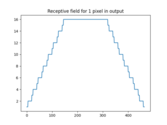
\includegraphics[width=\linewidth]{bilder/cpc-receptive-1p.png}
%%		\caption{Receptive field of standard CPC architecture from the paper for audio classification and number of times each pixel is used to calculate one pixel of the network output.}
%%		\label{explain}
%%		\centering
%%	\end{subfigure}
%%	\hfill
%%	\begin{subfigure}[t]{.4\textwidth}
%%		\centering
%%		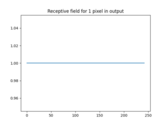
\includegraphics[width=\linewidth]{bilder/tcn-receptive-1p.png}
%%		\caption{Receptive field of a dilated convolutional net with fixed filtersize and exponentially increasing dilation and the number of times each pixel is used to calculate one pixel of the network output.}
%%		\label{explain}
%%	\end{subfigure}
%%	
%%	\medskip
%%	
%%	\begin{subfigure}[t]{.4\textwidth}
%%		\centering
%%		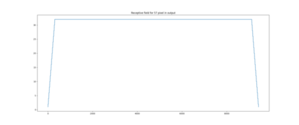
\includegraphics[width=\linewidth]{bilder/cpc-receptive-57p.png}
%%		\caption{Receptive field of standard CPC architecture from the paper for audio classification and number of times each pixel is used to calculate all 57 pixels of the network output.}
%%		\label{explain}
%%	\end{subfigure}
%%	\hfill
%%	\begin{subfigure}[t]{.4\textwidth}
%%		\centering
%%		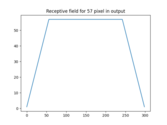
\includegraphics[width=\linewidth]{bilder/tcn-receptive-57p.png}
%%		\caption{Receptive field of a dilated convolutional net with fixed filtersize and exponentially increasing dilation and the number of times each pixel is used to calculate all 57 pixels of the network output.}
%%		\label{explain}
%%	\end{subfigure}
%%\end{figure}
%


\newpage
\begingroup
\makeatletter
\renewcommand\section{\@startsection{section}{3}{\z@}%
	{-3.25ex\@plus -1ex \@minus -.2ex}%
	{-1.5ex \@plus -.2ex}% Formerly 1.5ex \@plus .2ex
	{\normalfont\normalsize\bfseries}}
\renewcommand\subsection{\@startsection{subsection}{3}{\z@}%
	{-3.25ex\@plus -1ex \@minus -.2ex}%
	{-1.5ex \@plus -.2ex}% Formerly 1.5ex \@plus .2ex
	{\normalfont\normalsize\bfseries}}
\renewcommand\subsubsection{\@startsection{subsubsection}{3}{\z@}%
	{-3.25ex\@plus -1ex \@minus -.2ex}%
	{-1.5ex \@plus -.2ex}% Formerly 1.5ex \@plus .2ex
	{\normalfont\normalsize\bfseries}}
\renewcommand\paragraph{\@startsection{paragraph}{3}{\z@}%
	{-3.25ex\@plus -1ex \@minus -.2ex}%
	{-1.5ex \@plus -.2ex}% Formerly 1.5ex \@plus .2ex
	{\normalfont\normalsize\bfseries}}
\renewcommand\subparagraph{\@startsection{subparagraph}{3}{\z@}%
	{-3.25ex\@plus -1ex \@minus -.2ex}%
	{-1.5ex \@plus -.2ex}% Formerly 1.5ex \@plus .2ex
	{\normalfont\normalsize\bfseries}}
\makeatother
\lstdefinestyle{mystyle2}{
	backgroundcolor=\color{backcolour},   
	commentstyle=\color{codegreen},%
	keywordstyle=\color{magenta},%
	numberstyle=\tiny\color{codegray},
	stringstyle=\color{codepurple},
	basicstyle=\ttfamily\tiny, %\footnotesize,
	breakatwhitespace=false,         
	breaklines=true,                 
	captionpos=b,                    
	keepspaces=true,                 
	numbers=left,                    
	numbersep=5pt,                  
	showspaces=false,                
	showstringspaces=false,
	showtabs=false,                  
	tabsize=3
}
%TODO: printer
\definecolor{mycolorcode}{cmyk}{0.,0.,0.,0.95}
\definecolor{mycolorkeyword}{cmyk}{0.,0.,0.,1.}
\definecolor{mycolorcomment}{cmyk}{0.,0.,0.,0.8}
\definecolor{mycolorstring}{cmyk}{0.,0.,0.,0.8}
\definecolor{mycolorback}{cmyk}{0.,0.,0.,0.01}

\lstdefinestyle{mystyleblack}{
	backgroundcolor=\color{mycolorback},%\color{backcolour} 
	commentstyle=\color{mycolorcomment},%\color{codegreen}
	keywordstyle=\color{mycolorkeyword},%\color{magenta}
	numberstyle=\color{mycolorstring},%\tiny\color{codegray}
	stringstyle=\color{mycolorstring},%\color{codepurple}
	basicstyle=\ttfamily\tiny, %\footnotesize,
	breakatwhitespace=false,         
	breaklines=true,                 
	captionpos=b,                    
	keepspaces=true,    
	numbers=left,                    
	numbersep=5pt,                  
	showspaces=false,                
	showstringspaces=false,
	showtabs=false,                  
	tabsize=3
}
\lstset{
	style=mystyle2,
	literate=
	{á}{{\'a}}1 {é}{{\'e}}1 {í}{{\'i}}1 {ó}{{\'o}}1 {ú}{{\'u}}1
	{Á}{{\'A}}1 {É}{{\'E}}1 {Í}{{\'I}}1 {Ó}{{\'O}}1 {Ú}{{\'U}}1
	{à}{{\`a}}1 {è}{{\`e}}1 {ì}{{\`i}}1 {ò}{{\`o}}1 {ù}{{\`u}}1
	{À}{{\`A}}1 {È}{{\'E}}1 {Ì}{{\`I}}1 {Ò}{{\`O}}1 {Ù}{{\`U}}1
	{ä}{{\"a}}1 {ë}{{\"e}}1 {ï}{{\"i}}1 {ö}{{\"o}}1 {ü}{{\"u}}1
	{Ä}{{\"A}}1 {Ë}{{\"E}}1 {Ï}{{\"I}}1 {Ö}{{\"O}}1 {Ü}{{\"U}}1
	{â}{{\^a}}1 {ê}{{\^e}}1 {î}{{\^i}}1 {ô}{{\^o}}1 {û}{{\^u}}1
	{Â}{{\^A}}1 {Ê}{{\^E}}1 {Î}{{\^I}}1 {Ô}{{\^O}}1 {Û}{{\^U}}1
	{ã}{{\~a}}1 {ẽ}{{\~e}}1 {ĩ}{{\~i}}1 {õ}{{\~o}}1 {ũ}{{\~u}}1
	{Ã}{{\~A}}1 {Ẽ}{{\~E}}1 {Ĩ}{{\~I}}1 {Õ}{{\~O}}1 {Ũ}{{\~U}}1
	{œ}{{\oe}}1 {Œ}{{\OE}}1 {æ}{{\ae}}1 {Æ}{{\AE}}1 {ß}{{\ss}}1
	{ű}{{\H{u}}}1 {Ű}{{\H{U}}}1 {ő}{{\H{o}}}1 {Ő}{{\H{O}}}1
	{ç}{{\c c}}1 {Ç}{{\c C}}1 {ø}{{\o}}1 {å}{{\r a}}1 {Å}{{\r A}}1
}
\begin{myparindent}{0pt}

\noindent\section{Code} (folder)
	\noindent\subsection[architectures\_baseline\_challenge]{architectures\_baseline\_challenge} (folder)
\noindent\subsubsection[baseline\_FCN.py]{architectures\_baseline\_challenge -> baseline\_FCN.py} (code)
\lstinputlisting[language=Python]{"/home/julian/Downloads/Github/contrastive-predictive-coding/architectures_baseline_challenge/baseline_FCN.py"}
\noindent\subsubsection[baseline\_MLP.py]{architectures\_baseline\_challenge -> baseline\_MLP.py} (code)
\lstinputlisting[language=Python]{"/home/julian/Downloads/Github/contrastive-predictive-coding/architectures_baseline_challenge/baseline_MLP.py"}
\noindent\subsubsection[baseline\_TCN\_block.py]{architectures\_baseline\_challenge -> baseline\_TCN\_block.py} (code)
\lstinputlisting[language=Python]{"/home/julian/Downloads/Github/contrastive-predictive-coding/architectures_baseline_challenge/baseline_TCN_block.py"}
\noindent\subsubsection[baseline\_TCN\_down.py]{architectures\_baseline\_challenge -> baseline\_TCN\_down.py} (code)
\lstinputlisting[language=Python]{"/home/julian/Downloads/Github/contrastive-predictive-coding/architectures_baseline_challenge/baseline_TCN_down.py"}
\noindent\subsubsection[baseline\_TCN\_flatten.py]{architectures\_baseline\_challenge -> baseline\_TCN\_flatten.py} (code)
\lstinputlisting[language=Python]{"/home/julian/Downloads/Github/contrastive-predictive-coding/architectures_baseline_challenge/baseline_TCN_flatten.py"}
\noindent\subsubsection[baseline\_TCN\_last.py]{architectures\_baseline\_challenge -> baseline\_TCN\_last.py} (code)
\lstinputlisting[language=Python]{"/home/julian/Downloads/Github/contrastive-predictive-coding/architectures_baseline_challenge/baseline_TCN_last.py"}
\noindent\subsubsection[baseline\_alex.py]{architectures\_baseline\_challenge -> baseline\_alex.py} (code)
\lstinputlisting[language=Python]{"/home/julian/Downloads/Github/contrastive-predictive-coding/architectures_baseline_challenge/baseline_alex.py"}
\noindent\subsubsection[baseline\_alex\_v2.py]{architectures\_baseline\_challenge -> baseline\_alex\_v2.py} (code)
\lstinputlisting[language=Python]{"/home/julian/Downloads/Github/contrastive-predictive-coding/architectures_baseline_challenge/baseline_alex_v2.py"}
\noindent\subsubsection[baseline\_cnn\_v0.py]{architectures\_baseline\_challenge -> baseline\_cnn\_v0.py} (code)
\lstinputlisting[language=Python]{"/home/julian/Downloads/Github/contrastive-predictive-coding/architectures_baseline_challenge/baseline_cnn_v0.py"}
\noindent\subsubsection[baseline\_cnn\_v0\_1.py]{architectures\_baseline\_challenge -> baseline\_cnn\_v0\_1.py} (code)
\lstinputlisting[language=Python]{"/home/julian/Downloads/Github/contrastive-predictive-coding/architectures_baseline_challenge/baseline_cnn_v0_1.py"}
\noindent\subsubsection[baseline\_cnn\_v0\_2.py]{architectures\_baseline\_challenge -> baseline\_cnn\_v0\_2.py} (code)
\lstinputlisting[language=Python]{"/home/julian/Downloads/Github/contrastive-predictive-coding/architectures_baseline_challenge/baseline_cnn_v0_2.py"}
\noindent\subsubsection[baseline\_cnn\_v0\_3.py]{architectures\_baseline\_challenge -> baseline\_cnn\_v0\_3.py} (code)
\lstinputlisting[language=Python]{"/home/julian/Downloads/Github/contrastive-predictive-coding/architectures_baseline_challenge/baseline_cnn_v0_3.py"}
\noindent\subsubsection[baseline\_cnn\_v1.py]{architectures\_baseline\_challenge -> baseline\_cnn\_v1.py} (code)
\lstinputlisting[language=Python]{"/home/julian/Downloads/Github/contrastive-predictive-coding/architectures_baseline_challenge/baseline_cnn_v1.py"}
\noindent\subsubsection[baseline\_cnn\_v14.py]{architectures\_baseline\_challenge -> baseline\_cnn\_v14.py} (code)
\lstinputlisting[language=Python]{"/home/julian/Downloads/Github/contrastive-predictive-coding/architectures_baseline_challenge/baseline_cnn_v14.py"}
\noindent\subsubsection[baseline\_cnn\_v15.py]{architectures\_baseline\_challenge -> baseline\_cnn\_v15.py} (code)
\lstinputlisting[language=Python]{"/home/julian/Downloads/Github/contrastive-predictive-coding/architectures_baseline_challenge/baseline_cnn_v15.py"}
\noindent\subsubsection[baseline\_cnn\_v2.py]{architectures\_baseline\_challenge -> baseline\_cnn\_v2.py} (code)
\lstinputlisting[language=Python]{"/home/julian/Downloads/Github/contrastive-predictive-coding/architectures_baseline_challenge/baseline_cnn_v2.py"}
\noindent\subsubsection[baseline\_cnn\_v3.py]{architectures\_baseline\_challenge -> baseline\_cnn\_v3.py} (code)
\lstinputlisting[language=Python]{"/home/julian/Downloads/Github/contrastive-predictive-coding/architectures_baseline_challenge/baseline_cnn_v3.py"}
\noindent\subsubsection[baseline\_cnn\_v4.py]{architectures\_baseline\_challenge -> baseline\_cnn\_v4.py} (code)
\lstinputlisting[language=Python]{"/home/julian/Downloads/Github/contrastive-predictive-coding/architectures_baseline_challenge/baseline_cnn_v4.py"}
\noindent\subsubsection[baseline\_cnn\_v5.py]{architectures\_baseline\_challenge -> baseline\_cnn\_v5.py} (code)
\lstinputlisting[language=Python]{"/home/julian/Downloads/Github/contrastive-predictive-coding/architectures_baseline_challenge/baseline_cnn_v5.py"}
\noindent\subsubsection[baseline\_cnn\_v6.py]{architectures\_baseline\_challenge -> baseline\_cnn\_v6.py} (code)
\lstinputlisting[language=Python]{"/home/julian/Downloads/Github/contrastive-predictive-coding/architectures_baseline_challenge/baseline_cnn_v6.py"}
\noindent\subsubsection[baseline\_cnn\_v7.py]{architectures\_baseline\_challenge -> baseline\_cnn\_v7.py} (code)
\lstinputlisting[language=Python]{"/home/julian/Downloads/Github/contrastive-predictive-coding/architectures_baseline_challenge/baseline_cnn_v7.py"}
\noindent\subsubsection[baseline\_cnn\_v8.py]{architectures\_baseline\_challenge -> baseline\_cnn\_v8.py} (code)
\lstinputlisting[language=Python]{"/home/julian/Downloads/Github/contrastive-predictive-coding/architectures_baseline_challenge/baseline_cnn_v8.py"}
\noindent\subsubsection[baseline\_cnn\_v9.py]{architectures\_baseline\_challenge -> baseline\_cnn\_v9.py} (code)
\lstinputlisting[language=Python]{"/home/julian/Downloads/Github/contrastive-predictive-coding/architectures_baseline_challenge/baseline_cnn_v9.py"}
\noindent\subsubsection[baseline\_convencoder.py]{architectures\_baseline\_challenge -> baseline\_convencoder.py} (code)
\lstinputlisting[language=Python]{"/home/julian/Downloads/Github/contrastive-predictive-coding/architectures_baseline_challenge/baseline_convencoder.py"}
\noindent\subsubsection[baseline\_resnet.py]{architectures\_baseline\_challenge -> baseline\_resnet.py} (code)
\lstinputlisting[language=Python]{"/home/julian/Downloads/Github/contrastive-predictive-coding/architectures_baseline_challenge/baseline_resnet.py"}
\noindent\subsubsection[baseline\_rnn.py]{architectures\_baseline\_challenge -> baseline\_rnn.py} (code)
\lstinputlisting[language=Python]{"/home/julian/Downloads/Github/contrastive-predictive-coding/architectures_baseline_challenge/baseline_rnn.py"}
\noindent\subsubsection[baseline\_rnn\_simplest\_gru.py]{architectures\_baseline\_challenge -> baseline\_rnn\_simplest\_gru.py} (code)
\lstinputlisting[language=Python]{"/home/julian/Downloads/Github/contrastive-predictive-coding/architectures_baseline_challenge/baseline_rnn_simplest_gru.py"}
\noindent\subsubsection[baseline\_rnn\_simplest\_lstm.py]{architectures\_baseline\_challenge -> baseline\_rnn\_simplest\_lstm.py} (code)
\lstinputlisting[language=Python]{"/home/julian/Downloads/Github/contrastive-predictive-coding/architectures_baseline_challenge/baseline_rnn_simplest_lstm.py"}
\noindent\subsection[architectures\_cpc]{architectures\_cpc} (folder)
\noindent\subsubsection[cpc\_autoregressive\_hidden.py]{architectures\_cpc -> cpc\_autoregressive\_hidden.py} (code)
\lstinputlisting[language=Python]{"/home/julian/Downloads/Github/contrastive-predictive-coding/architectures_cpc/cpc_autoregressive_hidden.py"}
\noindent\subsubsection[cpc\_autoregressive\_v0.py]{architectures\_cpc -> cpc\_autoregressive\_v0.py} (code)
\lstinputlisting[language=Python]{"/home/julian/Downloads/Github/contrastive-predictive-coding/architectures_cpc/cpc_autoregressive_v0.py"}
\noindent\subsubsection[cpc\_base.py]{architectures\_cpc -> cpc\_base.py} (code)
\lstinputlisting[language=Python]{"/home/julian/Downloads/Github/contrastive-predictive-coding/architectures_cpc/cpc_base.py"}
\noindent\subsubsection[cpc\_combined.py]{architectures\_cpc -> cpc\_combined.py} (code)
\lstinputlisting[language=Python]{"/home/julian/Downloads/Github/contrastive-predictive-coding/architectures_cpc/cpc_combined.py"}
\noindent\subsubsection[cpc\_downstream\_cnn.py]{architectures\_cpc -> cpc\_downstream\_cnn.py} (code)
\lstinputlisting[language=Python]{"/home/julian/Downloads/Github/contrastive-predictive-coding/architectures_cpc/cpc_downstream_cnn.py"}
\noindent\subsubsection[cpc\_downstream\_latent\_average.py]{architectures\_cpc -> cpc\_downstream\_latent\_average.py} (code)
\lstinputlisting[language=Python]{"/home/julian/Downloads/Github/contrastive-predictive-coding/architectures_cpc/cpc_downstream_latent_average.py"}
\noindent\subsubsection[cpc\_downstream\_latent\_maximum.py]{architectures\_cpc -> cpc\_downstream\_latent\_maximum.py} (code)
\lstinputlisting[language=Python]{"/home/julian/Downloads/Github/contrastive-predictive-coding/architectures_cpc/cpc_downstream_latent_maximum.py"}
\noindent\subsubsection[cpc\_downstream\_model\_multitarget\_v1.py]{architectures\_cpc -> cpc\_downstream\_model\_multitarget\_v1.py} (code)
\lstinputlisting[language=Python]{"/home/julian/Downloads/Github/contrastive-predictive-coding/architectures_cpc/cpc_downstream_model_multitarget_v1.py"}
\noindent\subsubsection[cpc\_downstream\_model\_multitarget\_v2.py]{architectures\_cpc -> cpc\_downstream\_model\_multitarget\_v2.py} (code)
\lstinputlisting[language=Python]{"/home/julian/Downloads/Github/contrastive-predictive-coding/architectures_cpc/cpc_downstream_model_multitarget_v2.py"}
\noindent\subsubsection[cpc\_downstream\_only.py]{architectures\_cpc -> cpc\_downstream\_only.py} (code)
\lstinputlisting[language=Python]{"/home/julian/Downloads/Github/contrastive-predictive-coding/architectures_cpc/cpc_downstream_only.py"}
\noindent\subsubsection[cpc\_downstream\_twolinear.py]{architectures\_cpc -> cpc\_downstream\_twolinear.py} (code)
\lstinputlisting[language=Python]{"/home/julian/Downloads/Github/contrastive-predictive-coding/architectures_cpc/cpc_downstream_twolinear.py"}
\noindent\subsubsection[cpc\_downstream\_twolinear\_v2.py]{architectures\_cpc -> cpc\_downstream\_twolinear\_v2.py} (code)
\lstinputlisting[language=Python]{"/home/julian/Downloads/Github/contrastive-predictive-coding/architectures_cpc/cpc_downstream_twolinear_v2.py"}
\noindent\subsubsection[cpc\_encoder\_as\_strided.py]{architectures\_cpc -> cpc\_encoder\_as\_strided.py} (code)
\lstinputlisting[language=Python]{"/home/julian/Downloads/Github/contrastive-predictive-coding/architectures_cpc/cpc_encoder_as_strided.py"}
\noindent\subsubsection[cpc\_encoder\_decoder\_v2.py]{architectures\_cpc -> cpc\_encoder\_decoder\_v2.py} (code)
\lstinputlisting[language=Python]{"/home/julian/Downloads/Github/contrastive-predictive-coding/architectures_cpc/cpc_encoder_decoder_v2.py"}
\noindent\subsubsection[cpc\_encoder\_likev8.py]{architectures\_cpc -> cpc\_encoder\_likev8.py} (code)
\lstinputlisting[language=Python]{"/home/julian/Downloads/Github/contrastive-predictive-coding/architectures_cpc/cpc_encoder_likev8.py"}
\noindent\subsubsection[cpc\_encoder\_small.py]{architectures\_cpc -> cpc\_encoder\_small.py} (code)
\lstinputlisting[language=Python]{"/home/julian/Downloads/Github/contrastive-predictive-coding/architectures_cpc/cpc_encoder_small.py"}
\noindent\subsubsection[cpc\_encoder\_v0.py]{architectures\_cpc -> cpc\_encoder\_v0.py} (code)
\lstinputlisting[language=Python]{"/home/julian/Downloads/Github/contrastive-predictive-coding/architectures_cpc/cpc_encoder_v0.py"}
\noindent\subsubsection[cpc\_encoder\_v1.py]{architectures\_cpc -> cpc\_encoder\_v1.py} (code)
\lstinputlisting[language=Python]{"/home/julian/Downloads/Github/contrastive-predictive-coding/architectures_cpc/cpc_encoder_v1.py"}
\noindent\subsubsection[cpc\_encoder\_v2.py]{architectures\_cpc -> cpc\_encoder\_v2.py} (code)
\lstinputlisting[language=Python]{"/home/julian/Downloads/Github/contrastive-predictive-coding/architectures_cpc/cpc_encoder_v2.py"}
\noindent\subsubsection[cpc\_encoder\_v3.py]{architectures\_cpc -> cpc\_encoder\_v3.py} (code)
\lstinputlisting[language=Python]{"/home/julian/Downloads/Github/contrastive-predictive-coding/architectures_cpc/cpc_encoder_v3.py"}
\noindent\subsubsection[cpc\_encoder\_v4.py]{architectures\_cpc -> cpc\_encoder\_v4.py} (code)
\lstinputlisting[language=Python]{"/home/julian/Downloads/Github/contrastive-predictive-coding/architectures_cpc/cpc_encoder_v4.py"}
\noindent\subsubsection[cpc\_encoder\_vresnet.py]{architectures\_cpc -> cpc\_encoder\_vresnet.py} (code)
\lstinputlisting[language=Python]{"/home/julian/Downloads/Github/contrastive-predictive-coding/architectures_cpc/cpc_encoder_vresnet.py"}
\noindent\subsubsection[cpc\_intersect.py]{architectures\_cpc -> cpc\_intersect.py} (code)
\lstinputlisting[language=Python]{"/home/julian/Downloads/Github/contrastive-predictive-coding/architectures_cpc/cpc_intersect.py"}
\noindent\subsubsection[cpc\_intersect\_manylatents.py]{architectures\_cpc -> cpc\_intersect\_manylatents.py} (code)
\lstinputlisting[language=Python]{"/home/julian/Downloads/Github/contrastive-predictive-coding/architectures_cpc/cpc_intersect_manylatents.py"}
\noindent\subsubsection[cpc\_predictor\_nocontext.py]{architectures\_cpc -> cpc\_predictor\_nocontext.py} (code)
\lstinputlisting[language=Python]{"/home/julian/Downloads/Github/contrastive-predictive-coding/architectures_cpc/cpc_predictor_nocontext.py"}
\noindent\subsubsection[cpc\_predictor\_stacked.py]{architectures\_cpc -> cpc\_predictor\_stacked.py} (code)
\lstinputlisting[language=Python]{"/home/julian/Downloads/Github/contrastive-predictive-coding/architectures_cpc/cpc_predictor_stacked.py"}
\noindent\subsubsection[cpc\_predictor\_v0.py]{architectures\_cpc -> cpc\_predictor\_v0.py} (code)
\lstinputlisting[language=Python]{"/home/julian/Downloads/Github/contrastive-predictive-coding/architectures_cpc/cpc_predictor_v0.py"}
\noindent\subsubsection[cpc\_with\_decoder.py]{architectures\_cpc -> cpc\_with\_decoder.py} (code)
\lstinputlisting[language=Python]{"/home/julian/Downloads/Github/contrastive-predictive-coding/architectures_cpc/cpc_with_decoder.py"}
\noindent\subsection[architectures\_various]{architectures\_various} (folder)
\noindent\subsubsection[explain\_network.py]{architectures\_various -> explain\_network.py} (code)
\lstinputlisting[language=Python]{"/home/julian/Downloads/Github/contrastive-predictive-coding/architectures_various/explain_network.py"}
\noindent\subsubsection[explain\_network2.py]{architectures\_various -> explain\_network2.py} (code)
\lstinputlisting[language=Python]{"/home/julian/Downloads/Github/contrastive-predictive-coding/architectures_various/explain_network2.py"}
\noindent\subsection[deprecated]{deprecated} (folder)
\noindent\subsubsection[architectures\_baseline]{deprecated -> architectures\_baseline} (folder)
\noindent\paragraph[baseline\_cnn\_v0.py]{deprecated -> architectures\_baseline -> baseline\_cnn\_v0.py} (code)
\lstinputlisting[language=Python]{"/home/julian/Downloads/Github/contrastive-predictive-coding/deprecated/architectures_baseline/baseline_cnn_v0.py"}
\noindent\paragraph[baseline\_cnn\_v0\_1.py]{deprecated -> architectures\_baseline -> baseline\_cnn\_v0\_1.py} (code)
\lstinputlisting[language=Python]{"/home/julian/Downloads/Github/contrastive-predictive-coding/deprecated/architectures_baseline/baseline_cnn_v0_1.py"}
\noindent\paragraph[baseline\_cnn\_v0\_2.py]{deprecated -> architectures\_baseline -> baseline\_cnn\_v0\_2.py} (code)
\lstinputlisting[language=Python]{"/home/julian/Downloads/Github/contrastive-predictive-coding/deprecated/architectures_baseline/baseline_cnn_v0_2.py"}
\noindent\paragraph[baseline\_cnn\_v0\_3.py]{deprecated -> architectures\_baseline -> baseline\_cnn\_v0\_3.py} (code)
\lstinputlisting[language=Python]{"/home/julian/Downloads/Github/contrastive-predictive-coding/deprecated/architectures_baseline/baseline_cnn_v0_3.py"}
\noindent\paragraph[baseline\_cnn\_v1.py]{deprecated -> architectures\_baseline -> baseline\_cnn\_v1.py} (code)
\lstinputlisting[language=Python]{"/home/julian/Downloads/Github/contrastive-predictive-coding/deprecated/architectures_baseline/baseline_cnn_v1.py"}
\noindent\paragraph[baseline\_cnn\_v10.py]{deprecated -> architectures\_baseline -> baseline\_cnn\_v10.py} (code)
\lstinputlisting[language=Python]{"/home/julian/Downloads/Github/contrastive-predictive-coding/deprecated/architectures_baseline/baseline_cnn_v10.py"}
\noindent\paragraph[baseline\_cnn\_v11.py]{deprecated -> architectures\_baseline -> baseline\_cnn\_v11.py} (code)
\lstinputlisting[language=Python]{"/home/julian/Downloads/Github/contrastive-predictive-coding/deprecated/architectures_baseline/baseline_cnn_v11.py"}
\noindent\paragraph[baseline\_cnn\_v12.py]{deprecated -> architectures\_baseline -> baseline\_cnn\_v12.py} (code)
\lstinputlisting[language=Python]{"/home/julian/Downloads/Github/contrastive-predictive-coding/deprecated/architectures_baseline/baseline_cnn_v12.py"}
\noindent\paragraph[baseline\_cnn\_v13.py]{deprecated -> architectures\_baseline -> baseline\_cnn\_v13.py} (code)
\lstinputlisting[language=Python]{"/home/julian/Downloads/Github/contrastive-predictive-coding/deprecated/architectures_baseline/baseline_cnn_v13.py"}
\noindent\paragraph[baseline\_cnn\_v14.py]{deprecated -> architectures\_baseline -> baseline\_cnn\_v14.py} (code)
\lstinputlisting[language=Python]{"/home/julian/Downloads/Github/contrastive-predictive-coding/deprecated/architectures_baseline/baseline_cnn_v14.py"}
\noindent\paragraph[baseline\_cnn\_v2.py]{deprecated -> architectures\_baseline -> baseline\_cnn\_v2.py} (code)
\lstinputlisting[language=Python]{"/home/julian/Downloads/Github/contrastive-predictive-coding/deprecated/architectures_baseline/baseline_cnn_v2.py"}
\noindent\paragraph[baseline\_cnn\_v3.py]{deprecated -> architectures\_baseline -> baseline\_cnn\_v3.py} (code)
\lstinputlisting[language=Python]{"/home/julian/Downloads/Github/contrastive-predictive-coding/deprecated/architectures_baseline/baseline_cnn_v3.py"}
\noindent\paragraph[baseline\_cnn\_v4.py]{deprecated -> architectures\_baseline -> baseline\_cnn\_v4.py} (code)
\lstinputlisting[language=Python]{"/home/julian/Downloads/Github/contrastive-predictive-coding/deprecated/architectures_baseline/baseline_cnn_v4.py"}
\noindent\paragraph[baseline\_cnn\_v5.py]{deprecated -> architectures\_baseline -> baseline\_cnn\_v5.py} (code)
\lstinputlisting[language=Python]{"/home/julian/Downloads/Github/contrastive-predictive-coding/deprecated/architectures_baseline/baseline_cnn_v5.py"}
\noindent\paragraph[baseline\_cnn\_v6.py]{deprecated -> architectures\_baseline -> baseline\_cnn\_v6.py} (code)
\lstinputlisting[language=Python]{"/home/julian/Downloads/Github/contrastive-predictive-coding/deprecated/architectures_baseline/baseline_cnn_v6.py"}
\noindent\paragraph[baseline\_cnn\_v7.py]{deprecated -> architectures\_baseline -> baseline\_cnn\_v7.py} (code)
\lstinputlisting[language=Python]{"/home/julian/Downloads/Github/contrastive-predictive-coding/deprecated/architectures_baseline/baseline_cnn_v7.py"}
\noindent\paragraph[baseline\_cnn\_v8.py]{deprecated -> architectures\_baseline -> baseline\_cnn\_v8.py} (code)
\lstinputlisting[language=Python]{"/home/julian/Downloads/Github/contrastive-predictive-coding/deprecated/architectures_baseline/baseline_cnn_v8.py"}
\noindent\paragraph[baseline\_cnn\_v9.py]{deprecated -> architectures\_baseline -> baseline\_cnn\_v9.py} (code)
\lstinputlisting[language=Python]{"/home/julian/Downloads/Github/contrastive-predictive-coding/deprecated/architectures_baseline/baseline_cnn_v9.py"}
\noindent\paragraph[baseline\_convencoder.py]{deprecated -> architectures\_baseline -> baseline\_convencoder.py} (code)
\lstinputlisting[language=Python]{"/home/julian/Downloads/Github/contrastive-predictive-coding/deprecated/architectures_baseline/baseline_convencoder.py"}
\noindent\paragraph[baseline\_losses.py]{deprecated -> architectures\_baseline -> baseline\_losses.py} (code)
\lstinputlisting[language=Python]{"/home/julian/Downloads/Github/contrastive-predictive-coding/deprecated/architectures_baseline/baseline_losses.py"}
\noindent\subsubsection[cardio\_model\_v4.py]{deprecated -> cardio\_model\_v4.py} (code)
\lstinputlisting[language=Python]{"/home/julian/Downloads/Github/contrastive-predictive-coding/deprecated/cardio_model_v4.py"}
\noindent\subsubsection[cardio\_model\_v5.py]{deprecated -> cardio\_model\_v5.py} (code)
\lstinputlisting[language=Python]{"/home/julian/Downloads/Github/contrastive-predictive-coding/deprecated/cardio_model_v5.py"}
\noindent\subsubsection[cardio\_model\_v6.py]{deprecated -> cardio\_model\_v6.py} (code)
\lstinputlisting[language=Python]{"/home/julian/Downloads/Github/contrastive-predictive-coding/deprecated/cardio_model_v6.py"}
\noindent\subsubsection[cpc\_alpha.py]{deprecated -> cpc\_alpha.py} (code)
\lstinputlisting[language=Python]{"/home/julian/Downloads/Github/contrastive-predictive-coding/deprecated/cpc_alpha.py"}
\noindent\subsubsection[cpc\_decoder.py]{deprecated -> cpc\_decoder.py} (code)
\lstinputlisting[language=Python]{"/home/julian/Downloads/Github/contrastive-predictive-coding/deprecated/cpc_decoder.py"}
\noindent\subsubsection[cpc\_utils.py]{deprecated -> cpc\_utils.py} (code)
\lstinputlisting[language=Python]{"/home/julian/Downloads/Github/contrastive-predictive-coding/deprecated/cpc_utils.py"}
\noindent\subsubsection[data\_storage.py]{deprecated -> data\_storage.py} (code)
\lstinputlisting[language=Python]{"/home/julian/Downloads/Github/contrastive-predictive-coding/deprecated/data_storage.py"}
\noindent\subsubsection[downstream\_model.py]{deprecated -> downstream\_model.py} (code)
\lstinputlisting[language=Python]{"/home/julian/Downloads/Github/contrastive-predictive-coding/deprecated/downstream_model.py"}
\noindent\subsubsection[downstream\_model\_multitarget.py]{deprecated -> downstream\_model\_multitarget.py} (code)
\lstinputlisting[language=Python]{"/home/julian/Downloads/Github/contrastive-predictive-coding/deprecated/downstream_model_multitarget.py"}
\noindent\subsubsection[ecg\_datasets.py]{deprecated -> ecg\_datasets.py} (code)
\lstinputlisting[language=Python]{"/home/julian/Downloads/Github/contrastive-predictive-coding/deprecated/ecg_datasets.py"}
\noindent\subsubsection[main.py]{deprecated -> main.py} (code)
\lstinputlisting[language=Python]{"/home/julian/Downloads/Github/contrastive-predictive-coding/deprecated/main.py"}
\noindent\subsubsection[make\_clean\_data.py]{deprecated -> make\_clean\_data.py} (code)
\lstinputlisting[language=Python]{"/home/julian/Downloads/Github/contrastive-predictive-coding/deprecated/make_clean_data.py"}
\noindent\subsection[experiments]{experiments} (folder)
\noindent\subsubsection[create\_fewer\_labels\_data.py]{experiments -> create\_fewer\_labels\_data.py} (code)
\lstinputlisting[language=Python]{"/home/julian/Downloads/Github/contrastive-predictive-coding/experiments/create_fewer_labels_data.py"}
\noindent\subsubsection[create\_timeseries\_plots.py]{experiments -> create\_timeseries\_plots.py} (code)
\lstinputlisting[language=Python]{"/home/julian/Downloads/Github/contrastive-predictive-coding/experiments/create_timeseries_plots.py"}
\noindent\subsubsection[main\_get\_latents.py]{experiments -> main\_get\_latents.py} (code)
\lstinputlisting[language=Python]{"/home/julian/Downloads/Github/contrastive-predictive-coding/experiments/main_get_latents.py"}
\noindent\subsection[external]{external} (folder)
\noindent\subsubsection[tcn]{external -> tcn} (folder)
\noindent\paragraph[TCN]{external -> tcn -> TCN} (folder)
\noindent\subparagraph[tcn.py]{external -> tcn -> TCN -> tcn.py} (code)
\lstinputlisting[language=Python]{"/home/julian/Downloads/Github/contrastive-predictive-coding/external/tcn/TCN/tcn.py"}
\noindent\subsubsection[helper\_code.py]{external -> helper\_code.py} (code)
\lstinputlisting[language=Python]{"/home/julian/Downloads/Github/contrastive-predictive-coding/external/helper_code.py"}
\noindent\subsubsection[multi\_scale\_ori.py]{external -> multi\_scale\_ori.py} (code)
\lstinputlisting[language=Python]{"/home/julian/Downloads/Github/contrastive-predictive-coding/external/multi_scale_ori.py"}
\noindent\subsection[jupyter\_notebooks]{jupyter\_notebooks} (folder)
\noindent\subsubsection[Beat detection.py]{jupyter\_notebooks -> Beat detection.py} (code)
\lstinputlisting[language=Python]{"/home/julian/Downloads/Github/contrastive-predictive-coding/jupyter_notebooks/Beat detection.py"}
\noindent\subsubsection[CPC Loss Implementation Test.py]{jupyter\_notebooks -> CPC Loss Implementation Test.py} (code)
\lstinputlisting[language=Python]{"/home/julian/Downloads/Github/contrastive-predictive-coding/jupyter_notebooks/CPC Loss Implementation Test.py"}
\noindent\subsubsection[CPC Loss.py]{jupyter\_notebooks -> CPC Loss.py} (code)
\lstinputlisting[language=Python]{"/home/julian/Downloads/Github/contrastive-predictive-coding/jupyter_notebooks/CPC Loss.py"}
\noindent\subsubsection[Challenge Data Visualization.py]{jupyter\_notebooks -> Challenge Data Visualization.py} (code)
\lstinputlisting[language=Python]{"/home/julian/Downloads/Github/contrastive-predictive-coding/jupyter_notebooks/Challenge Data Visualization.py"}
\noindent\subsubsection[Export Code.py]{jupyter\_notebooks -> Export Code.py} (code)
\lstinputlisting[language=Python]{"/home/julian/Downloads/Github/contrastive-predictive-coding/jupyter_notebooks/Export Code.py"}
\noindent\subsubsection[Filter Attributes DataFrame.py]{jupyter\_notebooks -> Filter Attributes DataFrame.py} (code)
\lstinputlisting[language=Python]{"/home/julian/Downloads/Github/contrastive-predictive-coding/jupyter_notebooks/Filter Attributes DataFrame.py"}
\noindent\subsubsection[InfoNCE Loss Psuedo.py]{jupyter\_notebooks -> InfoNCE Loss Psuedo.py} (code)
\lstinputlisting[language=Python]{"/home/julian/Downloads/Github/contrastive-predictive-coding/jupyter_notebooks/InfoNCE Loss Psuedo.py"}
\noindent\subsubsection[MIT data.py]{jupyter\_notebooks -> MIT data.py} (code)
\lstinputlisting[language=Python]{"/home/julian/Downloads/Github/contrastive-predictive-coding/jupyter_notebooks/MIT data.py"}
\noindent\subsubsection[Model Gradient-Prediction Scatter.py]{jupyter\_notebooks -> Model Gradient-Prediction Scatter.py} (code)
\lstinputlisting[language=Python]{"/home/julian/Downloads/Github/contrastive-predictive-coding/jupyter_notebooks/Model Gradient-Prediction Scatter.py"}
\noindent\subsubsection[PTB PCA.py]{jupyter\_notebooks -> PTB PCA.py} (code)
\lstinputlisting[language=Python]{"/home/julian/Downloads/Github/contrastive-predictive-coding/jupyter_notebooks/PTB PCA.py"}
\noindent\subsubsection[PTBxl data.py]{jupyter\_notebooks -> PTBxl data.py} (code)
\lstinputlisting[language=Python]{"/home/julian/Downloads/Github/contrastive-predictive-coding/jupyter_notebooks/PTBxl data.py"}
\noindent\subsubsection[Parallel Coordinates.py]{jupyter\_notebooks -> Parallel Coordinates.py} (code)
\lstinputlisting[language=Python]{"/home/julian/Downloads/Github/contrastive-predictive-coding/jupyter_notebooks/Parallel Coordinates.py"}
\noindent\subsubsection[Physionet Hz Converter.py]{jupyter\_notebooks -> Physionet Hz Converter.py} (code)
\lstinputlisting[language=Python]{"/home/julian/Downloads/Github/contrastive-predictive-coding/jupyter_notebooks/Physionet Hz Converter.py"}
\noindent\subsubsection[Precision Recall.py]{jupyter\_notebooks -> Precision Recall.py} (code)
\lstinputlisting[language=Python]{"/home/julian/Downloads/Github/contrastive-predictive-coding/jupyter_notebooks/Precision Recall.py"}
\noindent\subsubsection[ROC.py]{jupyter\_notebooks -> ROC.py} (code)
\lstinputlisting[language=Python]{"/home/julian/Downloads/Github/contrastive-predictive-coding/jupyter_notebooks/ROC.py"}
\noindent\subsubsection[Sinus Generator.py]{jupyter\_notebooks -> Sinus Generator.py} (code)
\lstinputlisting[language=Python]{"/home/julian/Downloads/Github/contrastive-predictive-coding/jupyter_notebooks/Sinus Generator.py"}
\noindent\subsubsection[TSNE.py]{jupyter\_notebooks -> TSNE.py} (code)
\lstinputlisting[language=Python]{"/home/julian/Downloads/Github/contrastive-predictive-coding/jupyter_notebooks/TSNE.py"}
\noindent\subsection[logs]{logs} (folder)
\noindent\subsection[models\_evaluated\_filtered\_csv]{models\_evaluated\_filtered\_csv} (folder)
\noindent\subsubsection[old]{models\_evaluated\_filtered\_csv -> old} (folder)
\noindent\subsection[util]{util} (folder)
\noindent\subsubsection[data]{util -> data} (folder)
\noindent\paragraph[clear\_h5\_files.py]{util -> data -> clear\_h5\_files.py} (code)
\lstinputlisting[language=Python]{"/home/julian/Downloads/Github/contrastive-predictive-coding/util/data/clear_h5_files.py"}
\noindent\paragraph[dataframe\_factory.py]{util -> data -> dataframe\_factory.py} (code)
\lstinputlisting[language=Python]{"/home/julian/Downloads/Github/contrastive-predictive-coding/util/data/dataframe_factory.py"}
\noindent\paragraph[dataset\_container.py]{util -> data -> dataset\_container.py} (code)
\lstinputlisting[language=Python]{"/home/julian/Downloads/Github/contrastive-predictive-coding/util/data/dataset_container.py"}
\noindent\paragraph[ecg\_data.py]{util -> data -> ecg\_data.py} (code)
\lstinputlisting[language=Python]{"/home/julian/Downloads/Github/contrastive-predictive-coding/util/data/ecg_data.py"}
\noindent\paragraph[ecg\_datasets2.py]{util -> data -> ecg\_datasets2.py} (code)
\lstinputlisting[language=Python]{"/home/julian/Downloads/Github/contrastive-predictive-coding/util/data/ecg_datasets2.py"}
\noindent\paragraph[ecg\_datasets3.py]{util -> data -> ecg\_datasets3.py} (code)
\lstinputlisting[language=Python]{"/home/julian/Downloads/Github/contrastive-predictive-coding/util/data/ecg_datasets3.py"}
\noindent\paragraph[ptbxl\_data.py]{util -> data -> ptbxl\_data.py} (code)
\lstinputlisting[language=Python]{"/home/julian/Downloads/Github/contrastive-predictive-coding/util/data/ptbxl_data.py"}
\noindent\subsubsection[metrics]{util -> metrics} (folder)
\noindent\paragraph[baseline\_losses.py]{util -> metrics -> baseline\_losses.py} (code)
\lstinputlisting[language=Python]{"/home/julian/Downloads/Github/contrastive-predictive-coding/util/metrics/baseline_losses.py"}
\noindent\paragraph[metrics.py]{util -> metrics -> metrics.py} (code)
\lstinputlisting[language=Python]{"/home/julian/Downloads/Github/contrastive-predictive-coding/util/metrics/metrics.py"}
\noindent\paragraph[training\_metrics.py]{util -> metrics -> training\_metrics.py} (code)
\lstinputlisting[language=Python]{"/home/julian/Downloads/Github/contrastive-predictive-coding/util/metrics/training_metrics.py"}
\noindent\subsubsection[utility]{util -> utility} (folder)
\noindent\paragraph[dict\_utils.py]{util -> utility -> dict\_utils.py} (code)
\lstinputlisting[language=Python]{"/home/julian/Downloads/Github/contrastive-predictive-coding/util/utility/dict_utils.py"}
\noindent\paragraph[extract\_trained\_model\_attributes.py]{util -> utility -> extract\_trained\_model\_attributes.py} (code)
\lstinputlisting[language=Python]{"/home/julian/Downloads/Github/contrastive-predictive-coding/util/utility/extract_trained_model_attributes.py"}
\noindent\paragraph[full\_class\_name.py]{util -> utility -> full\_class\_name.py} (code)
\lstinputlisting[language=Python]{"/home/julian/Downloads/Github/contrastive-predictive-coding/util/utility/full_class_name.py"}
\noindent\paragraph[layer\_calculations.py]{util -> utility -> layer\_calculations.py} (code)
\lstinputlisting[language=Python]{"/home/julian/Downloads/Github/contrastive-predictive-coding/util/utility/layer_calculations.py"}
\noindent\paragraph[print\_layer.py]{util -> utility -> print\_layer.py} (code)
\lstinputlisting[language=Python]{"/home/julian/Downloads/Github/contrastive-predictive-coding/util/utility/print_layer.py"}
\noindent\paragraph[sparse\_print.py]{util -> utility -> sparse\_print.py} (code)
\lstinputlisting[language=Python]{"/home/julian/Downloads/Github/contrastive-predictive-coding/util/utility/sparse_print.py"}
\noindent\paragraph[timestamp.py]{util -> utility -> timestamp.py} (code)
\lstinputlisting[language=Python]{"/home/julian/Downloads/Github/contrastive-predictive-coding/util/utility/timestamp.py"}
\noindent\subsubsection[visualize]{util -> visualize} (folder)
\noindent\paragraph[layer\_visualization.py]{util -> visualize -> layer\_visualization.py} (code)
\lstinputlisting[language=Python]{"/home/julian/Downloads/Github/contrastive-predictive-coding/util/visualize/layer_visualization.py"}
\noindent\paragraph[plot\_metrics.py]{util -> visualize -> plot\_metrics.py} (code)
\lstinputlisting[language=Python]{"/home/julian/Downloads/Github/contrastive-predictive-coding/util/visualize/plot_metrics.py"}
\noindent\paragraph[timeseries\_to\_image\_converter.py]{util -> visualize -> timeseries\_to\_image\_converter.py} (code)
\lstinputlisting[language=Python]{"/home/julian/Downloads/Github/contrastive-predictive-coding/util/visualize/timeseries_to_image_converter.py"}
\noindent\subsubsection[store\_models.py]{util -> store\_models.py} (code)
\lstinputlisting[language=Python]{"/home/julian/Downloads/Github/contrastive-predictive-coding/util/store_models.py"}
\noindent\subsection[main\_cpc\_benchmark\_test.py]{main\_cpc\_benchmark\_test.py} (code)
\lstinputlisting[language=Python]{"/home/julian/Downloads/Github/contrastive-predictive-coding/main_cpc_benchmark_test.py"}
\noindent\subsection[main\_cpc\_benchmark\_train.py]{main\_cpc\_benchmark\_train.py} (code)
\lstinputlisting[language=Python]{"/home/julian/Downloads/Github/contrastive-predictive-coding/main_cpc_benchmark_train.py"}
\noindent\subsection[main\_cpc\_explain.py]{main\_cpc\_explain.py} (code)
\lstinputlisting[language=Python]{"/home/julian/Downloads/Github/contrastive-predictive-coding/main_cpc_explain.py"}
\noindent\subsection[main\_cpc\_explain\_gradcam.py]{main\_cpc\_explain\_gradcam.py} (code)
\lstinputlisting[language=Python]{"/home/julian/Downloads/Github/contrastive-predictive-coding/main_cpc_explain_gradcam.py"}
\noindent\subsection[main\_produce\_plots\_for\_tested\_models.py]{main\_produce\_plots\_for\_tested\_models.py} (code)
\lstinputlisting[language=Python]{"/home/julian/Downloads/Github/contrastive-predictive-coding/main_produce_plots_for_tested_models.py"}
\end{myparindent}
\endgroup
%\startcontents
%\printcontents{}{0}[5]{}
%\newpage
\begingroup
\makeatletter
\renewcommand\section{\@startsection{section}{3}{\z@}%
	{-3.25ex\@plus -1ex \@minus -.2ex}%
	{-1.5ex \@plus -.2ex}% Formerly 1.5ex \@plus .2ex
	{\normalfont\normalsize\bfseries}}
\renewcommand\subsection{\@startsection{subsection}{3}{\z@}%
	{-3.25ex\@plus -1ex \@minus -.2ex}%
	{-1.5ex \@plus -.2ex}% Formerly 1.5ex \@plus .2ex
	{\normalfont\normalsize\bfseries}}
\renewcommand\subsubsection{\@startsection{subsubsection}{3}{\z@}%
	{-3.25ex\@plus -1ex \@minus -.2ex}%
	{-1.5ex \@plus -.2ex}% Formerly 1.5ex \@plus .2ex
	{\normalfont\normalsize\bfseries}}
\renewcommand\paragraph{\@startsection{paragraph}{3}{\z@}%
	{-3.25ex\@plus -1ex \@minus -.2ex}%
	{-1.5ex \@plus -.2ex}% Formerly 1.5ex \@plus .2ex
	{\normalfont\normalsize\bfseries}}
\renewcommand\subparagraph{\@startsection{subparagraph}{3}{\z@}%
	{-3.25ex\@plus -1ex \@minus -.2ex}%
	{-1.5ex \@plus -.2ex}% Formerly 1.5ex \@plus .2ex
	{\normalfont\normalsize\bfseries}}
\makeatother
\lstdefinestyle{mystyle2}{
	backgroundcolor=\color{backcolour},   
	commentstyle=\color{codegreen},%
	keywordstyle=\color{magenta},%
	numberstyle=\tiny\color{codegray},
	stringstyle=\color{codepurple},
	basicstyle=\ttfamily\tiny, %\footnotesize,
	breakatwhitespace=false,         
	breaklines=true,                 
	captionpos=b,                    
	keepspaces=true,                 
	numbers=left,                    
	numbersep=5pt,                  
	showspaces=false,                
	showstringspaces=false,
	showtabs=false,                  
	tabsize=3
}
%TODO: printer
\definecolor{mycolorcode}{cmyk}{0.,0.,0.,0.95}
\definecolor{mycolorkeyword}{cmyk}{0.,0.,0.,1.}
\definecolor{mycolorcomment}{cmyk}{0.,0.,0.,0.8}
\definecolor{mycolorstring}{cmyk}{0.,0.,0.,0.8}
\definecolor{mycolorback}{cmyk}{0.,0.,0.,0.01}

\lstdefinestyle{mystyleblack}{
	backgroundcolor=\color{mycolorback},%\color{backcolour} 
	commentstyle=\color{mycolorcomment},%\color{codegreen}
	keywordstyle=\color{mycolorkeyword},%\color{magenta}
	numberstyle=\color{mycolorstring},%\tiny\color{codegray}
	stringstyle=\color{mycolorstring},%\color{codepurple}
	basicstyle=\ttfamily\tiny, %\footnotesize,
	breakatwhitespace=false,         
	breaklines=true,                 
	captionpos=b,                    
	keepspaces=true,    
	numbers=left,                    
	numbersep=5pt,                  
	showspaces=false,                
	showstringspaces=false,
	showtabs=false,                  
	tabsize=3
}
\lstset{
	style=mystyle2,
	literate=
	{á}{{\'a}}1 {é}{{\'e}}1 {í}{{\'i}}1 {ó}{{\'o}}1 {ú}{{\'u}}1
	{Á}{{\'A}}1 {É}{{\'E}}1 {Í}{{\'I}}1 {Ó}{{\'O}}1 {Ú}{{\'U}}1
	{à}{{\`a}}1 {è}{{\`e}}1 {ì}{{\`i}}1 {ò}{{\`o}}1 {ù}{{\`u}}1
	{À}{{\`A}}1 {È}{{\'E}}1 {Ì}{{\`I}}1 {Ò}{{\`O}}1 {Ù}{{\`U}}1
	{ä}{{\"a}}1 {ë}{{\"e}}1 {ï}{{\"i}}1 {ö}{{\"o}}1 {ü}{{\"u}}1
	{Ä}{{\"A}}1 {Ë}{{\"E}}1 {Ï}{{\"I}}1 {Ö}{{\"O}}1 {Ü}{{\"U}}1
	{â}{{\^a}}1 {ê}{{\^e}}1 {î}{{\^i}}1 {ô}{{\^o}}1 {û}{{\^u}}1
	{Â}{{\^A}}1 {Ê}{{\^E}}1 {Î}{{\^I}}1 {Ô}{{\^O}}1 {Û}{{\^U}}1
	{ã}{{\~a}}1 {ẽ}{{\~e}}1 {ĩ}{{\~i}}1 {õ}{{\~o}}1 {ũ}{{\~u}}1
	{Ã}{{\~A}}1 {Ẽ}{{\~E}}1 {Ĩ}{{\~I}}1 {Õ}{{\~O}}1 {Ũ}{{\~U}}1
	{œ}{{\oe}}1 {Œ}{{\OE}}1 {æ}{{\ae}}1 {Æ}{{\AE}}1 {ß}{{\ss}}1
	{ű}{{\H{u}}}1 {Ű}{{\H{U}}}1 {ő}{{\H{o}}}1 {Ő}{{\H{O}}}1
	{ç}{{\c c}}1 {Ç}{{\c C}}1 {ø}{{\o}}1 {å}{{\r a}}1 {Å}{{\r A}}1
}
\begin{myparindent}{0pt}

\noindent\section{Code} (folder)
	\noindent\subsection[architectures\_baseline\_challenge]{architectures\_baseline\_challenge} (folder)
\noindent\subsubsection[baseline\_FCN.py]{architectures\_baseline\_challenge -> baseline\_FCN.py} (code)
\lstinputlisting[language=Python]{"/home/julian/Downloads/Github/contrastive-predictive-coding/architectures_baseline_challenge/baseline_FCN.py"}
\noindent\subsubsection[baseline\_MLP.py]{architectures\_baseline\_challenge -> baseline\_MLP.py} (code)
\lstinputlisting[language=Python]{"/home/julian/Downloads/Github/contrastive-predictive-coding/architectures_baseline_challenge/baseline_MLP.py"}
\noindent\subsubsection[baseline\_TCN\_block.py]{architectures\_baseline\_challenge -> baseline\_TCN\_block.py} (code)
\lstinputlisting[language=Python]{"/home/julian/Downloads/Github/contrastive-predictive-coding/architectures_baseline_challenge/baseline_TCN_block.py"}
\noindent\subsubsection[baseline\_TCN\_down.py]{architectures\_baseline\_challenge -> baseline\_TCN\_down.py} (code)
\lstinputlisting[language=Python]{"/home/julian/Downloads/Github/contrastive-predictive-coding/architectures_baseline_challenge/baseline_TCN_down.py"}
\noindent\subsubsection[baseline\_TCN\_flatten.py]{architectures\_baseline\_challenge -> baseline\_TCN\_flatten.py} (code)
\lstinputlisting[language=Python]{"/home/julian/Downloads/Github/contrastive-predictive-coding/architectures_baseline_challenge/baseline_TCN_flatten.py"}
\noindent\subsubsection[baseline\_TCN\_last.py]{architectures\_baseline\_challenge -> baseline\_TCN\_last.py} (code)
\lstinputlisting[language=Python]{"/home/julian/Downloads/Github/contrastive-predictive-coding/architectures_baseline_challenge/baseline_TCN_last.py"}
\noindent\subsubsection[baseline\_alex.py]{architectures\_baseline\_challenge -> baseline\_alex.py} (code)
\lstinputlisting[language=Python]{"/home/julian/Downloads/Github/contrastive-predictive-coding/architectures_baseline_challenge/baseline_alex.py"}
\noindent\subsubsection[baseline\_alex\_v2.py]{architectures\_baseline\_challenge -> baseline\_alex\_v2.py} (code)
\lstinputlisting[language=Python]{"/home/julian/Downloads/Github/contrastive-predictive-coding/architectures_baseline_challenge/baseline_alex_v2.py"}
\noindent\subsubsection[baseline\_cnn\_v0.py]{architectures\_baseline\_challenge -> baseline\_cnn\_v0.py} (code)
\lstinputlisting[language=Python]{"/home/julian/Downloads/Github/contrastive-predictive-coding/architectures_baseline_challenge/baseline_cnn_v0.py"}
\noindent\subsubsection[baseline\_cnn\_v0\_1.py]{architectures\_baseline\_challenge -> baseline\_cnn\_v0\_1.py} (code)
\lstinputlisting[language=Python]{"/home/julian/Downloads/Github/contrastive-predictive-coding/architectures_baseline_challenge/baseline_cnn_v0_1.py"}
\noindent\subsubsection[baseline\_cnn\_v0\_2.py]{architectures\_baseline\_challenge -> baseline\_cnn\_v0\_2.py} (code)
\lstinputlisting[language=Python]{"/home/julian/Downloads/Github/contrastive-predictive-coding/architectures_baseline_challenge/baseline_cnn_v0_2.py"}
\noindent\subsubsection[baseline\_cnn\_v0\_3.py]{architectures\_baseline\_challenge -> baseline\_cnn\_v0\_3.py} (code)
\lstinputlisting[language=Python]{"/home/julian/Downloads/Github/contrastive-predictive-coding/architectures_baseline_challenge/baseline_cnn_v0_3.py"}
\noindent\subsubsection[baseline\_cnn\_v1.py]{architectures\_baseline\_challenge -> baseline\_cnn\_v1.py} (code)
\lstinputlisting[language=Python]{"/home/julian/Downloads/Github/contrastive-predictive-coding/architectures_baseline_challenge/baseline_cnn_v1.py"}
\noindent\subsubsection[baseline\_cnn\_v14.py]{architectures\_baseline\_challenge -> baseline\_cnn\_v14.py} (code)
\lstinputlisting[language=Python]{"/home/julian/Downloads/Github/contrastive-predictive-coding/architectures_baseline_challenge/baseline_cnn_v14.py"}
\noindent\subsubsection[baseline\_cnn\_v15.py]{architectures\_baseline\_challenge -> baseline\_cnn\_v15.py} (code)
\lstinputlisting[language=Python]{"/home/julian/Downloads/Github/contrastive-predictive-coding/architectures_baseline_challenge/baseline_cnn_v15.py"}
\noindent\subsubsection[baseline\_cnn\_v2.py]{architectures\_baseline\_challenge -> baseline\_cnn\_v2.py} (code)
\lstinputlisting[language=Python]{"/home/julian/Downloads/Github/contrastive-predictive-coding/architectures_baseline_challenge/baseline_cnn_v2.py"}
\noindent\subsubsection[baseline\_cnn\_v3.py]{architectures\_baseline\_challenge -> baseline\_cnn\_v3.py} (code)
\lstinputlisting[language=Python]{"/home/julian/Downloads/Github/contrastive-predictive-coding/architectures_baseline_challenge/baseline_cnn_v3.py"}
\noindent\subsubsection[baseline\_cnn\_v4.py]{architectures\_baseline\_challenge -> baseline\_cnn\_v4.py} (code)
\lstinputlisting[language=Python]{"/home/julian/Downloads/Github/contrastive-predictive-coding/architectures_baseline_challenge/baseline_cnn_v4.py"}
\noindent\subsubsection[baseline\_cnn\_v5.py]{architectures\_baseline\_challenge -> baseline\_cnn\_v5.py} (code)
\lstinputlisting[language=Python]{"/home/julian/Downloads/Github/contrastive-predictive-coding/architectures_baseline_challenge/baseline_cnn_v5.py"}
\noindent\subsubsection[baseline\_cnn\_v6.py]{architectures\_baseline\_challenge -> baseline\_cnn\_v6.py} (code)
\lstinputlisting[language=Python]{"/home/julian/Downloads/Github/contrastive-predictive-coding/architectures_baseline_challenge/baseline_cnn_v6.py"}
\noindent\subsubsection[baseline\_cnn\_v7.py]{architectures\_baseline\_challenge -> baseline\_cnn\_v7.py} (code)
\lstinputlisting[language=Python]{"/home/julian/Downloads/Github/contrastive-predictive-coding/architectures_baseline_challenge/baseline_cnn_v7.py"}
\noindent\subsubsection[baseline\_cnn\_v8.py]{architectures\_baseline\_challenge -> baseline\_cnn\_v8.py} (code)
\lstinputlisting[language=Python]{"/home/julian/Downloads/Github/contrastive-predictive-coding/architectures_baseline_challenge/baseline_cnn_v8.py"}
\noindent\subsubsection[baseline\_cnn\_v9.py]{architectures\_baseline\_challenge -> baseline\_cnn\_v9.py} (code)
\lstinputlisting[language=Python]{"/home/julian/Downloads/Github/contrastive-predictive-coding/architectures_baseline_challenge/baseline_cnn_v9.py"}
\noindent\subsubsection[baseline\_convencoder.py]{architectures\_baseline\_challenge -> baseline\_convencoder.py} (code)
\lstinputlisting[language=Python]{"/home/julian/Downloads/Github/contrastive-predictive-coding/architectures_baseline_challenge/baseline_convencoder.py"}
\noindent\subsubsection[baseline\_resnet.py]{architectures\_baseline\_challenge -> baseline\_resnet.py} (code)
\lstinputlisting[language=Python]{"/home/julian/Downloads/Github/contrastive-predictive-coding/architectures_baseline_challenge/baseline_resnet.py"}
\noindent\subsubsection[baseline\_rnn.py]{architectures\_baseline\_challenge -> baseline\_rnn.py} (code)
\lstinputlisting[language=Python]{"/home/julian/Downloads/Github/contrastive-predictive-coding/architectures_baseline_challenge/baseline_rnn.py"}
\noindent\subsubsection[baseline\_rnn\_simplest\_gru.py]{architectures\_baseline\_challenge -> baseline\_rnn\_simplest\_gru.py} (code)
\lstinputlisting[language=Python]{"/home/julian/Downloads/Github/contrastive-predictive-coding/architectures_baseline_challenge/baseline_rnn_simplest_gru.py"}
\noindent\subsubsection[baseline\_rnn\_simplest\_lstm.py]{architectures\_baseline\_challenge -> baseline\_rnn\_simplest\_lstm.py} (code)
\lstinputlisting[language=Python]{"/home/julian/Downloads/Github/contrastive-predictive-coding/architectures_baseline_challenge/baseline_rnn_simplest_lstm.py"}
\noindent\subsection[architectures\_cpc]{architectures\_cpc} (folder)
\noindent\subsubsection[cpc\_autoregressive\_hidden.py]{architectures\_cpc -> cpc\_autoregressive\_hidden.py} (code)
\lstinputlisting[language=Python]{"/home/julian/Downloads/Github/contrastive-predictive-coding/architectures_cpc/cpc_autoregressive_hidden.py"}
\noindent\subsubsection[cpc\_autoregressive\_v0.py]{architectures\_cpc -> cpc\_autoregressive\_v0.py} (code)
\lstinputlisting[language=Python]{"/home/julian/Downloads/Github/contrastive-predictive-coding/architectures_cpc/cpc_autoregressive_v0.py"}
\noindent\subsubsection[cpc\_base.py]{architectures\_cpc -> cpc\_base.py} (code)
\lstinputlisting[language=Python]{"/home/julian/Downloads/Github/contrastive-predictive-coding/architectures_cpc/cpc_base.py"}
\noindent\subsubsection[cpc\_combined.py]{architectures\_cpc -> cpc\_combined.py} (code)
\lstinputlisting[language=Python]{"/home/julian/Downloads/Github/contrastive-predictive-coding/architectures_cpc/cpc_combined.py"}
\noindent\subsubsection[cpc\_downstream\_cnn.py]{architectures\_cpc -> cpc\_downstream\_cnn.py} (code)
\lstinputlisting[language=Python]{"/home/julian/Downloads/Github/contrastive-predictive-coding/architectures_cpc/cpc_downstream_cnn.py"}
\noindent\subsubsection[cpc\_downstream\_latent\_average.py]{architectures\_cpc -> cpc\_downstream\_latent\_average.py} (code)
\lstinputlisting[language=Python]{"/home/julian/Downloads/Github/contrastive-predictive-coding/architectures_cpc/cpc_downstream_latent_average.py"}
\noindent\subsubsection[cpc\_downstream\_latent\_maximum.py]{architectures\_cpc -> cpc\_downstream\_latent\_maximum.py} (code)
\lstinputlisting[language=Python]{"/home/julian/Downloads/Github/contrastive-predictive-coding/architectures_cpc/cpc_downstream_latent_maximum.py"}
\noindent\subsubsection[cpc\_downstream\_model\_multitarget\_v1.py]{architectures\_cpc -> cpc\_downstream\_model\_multitarget\_v1.py} (code)
\lstinputlisting[language=Python]{"/home/julian/Downloads/Github/contrastive-predictive-coding/architectures_cpc/cpc_downstream_model_multitarget_v1.py"}
\noindent\subsubsection[cpc\_downstream\_model\_multitarget\_v2.py]{architectures\_cpc -> cpc\_downstream\_model\_multitarget\_v2.py} (code)
\lstinputlisting[language=Python]{"/home/julian/Downloads/Github/contrastive-predictive-coding/architectures_cpc/cpc_downstream_model_multitarget_v2.py"}
\noindent\subsubsection[cpc\_downstream\_only.py]{architectures\_cpc -> cpc\_downstream\_only.py} (code)
\lstinputlisting[language=Python]{"/home/julian/Downloads/Github/contrastive-predictive-coding/architectures_cpc/cpc_downstream_only.py"}
\noindent\subsubsection[cpc\_downstream\_twolinear.py]{architectures\_cpc -> cpc\_downstream\_twolinear.py} (code)
\lstinputlisting[language=Python]{"/home/julian/Downloads/Github/contrastive-predictive-coding/architectures_cpc/cpc_downstream_twolinear.py"}
\noindent\subsubsection[cpc\_downstream\_twolinear\_v2.py]{architectures\_cpc -> cpc\_downstream\_twolinear\_v2.py} (code)
\lstinputlisting[language=Python]{"/home/julian/Downloads/Github/contrastive-predictive-coding/architectures_cpc/cpc_downstream_twolinear_v2.py"}
\noindent\subsubsection[cpc\_encoder\_as\_strided.py]{architectures\_cpc -> cpc\_encoder\_as\_strided.py} (code)
\lstinputlisting[language=Python]{"/home/julian/Downloads/Github/contrastive-predictive-coding/architectures_cpc/cpc_encoder_as_strided.py"}
\noindent\subsubsection[cpc\_encoder\_decoder\_v2.py]{architectures\_cpc -> cpc\_encoder\_decoder\_v2.py} (code)
\lstinputlisting[language=Python]{"/home/julian/Downloads/Github/contrastive-predictive-coding/architectures_cpc/cpc_encoder_decoder_v2.py"}
\noindent\subsubsection[cpc\_encoder\_likev8.py]{architectures\_cpc -> cpc\_encoder\_likev8.py} (code)
\lstinputlisting[language=Python]{"/home/julian/Downloads/Github/contrastive-predictive-coding/architectures_cpc/cpc_encoder_likev8.py"}
\noindent\subsubsection[cpc\_encoder\_small.py]{architectures\_cpc -> cpc\_encoder\_small.py} (code)
\lstinputlisting[language=Python]{"/home/julian/Downloads/Github/contrastive-predictive-coding/architectures_cpc/cpc_encoder_small.py"}
\noindent\subsubsection[cpc\_encoder\_v0.py]{architectures\_cpc -> cpc\_encoder\_v0.py} (code)
\lstinputlisting[language=Python]{"/home/julian/Downloads/Github/contrastive-predictive-coding/architectures_cpc/cpc_encoder_v0.py"}
\noindent\subsubsection[cpc\_encoder\_v1.py]{architectures\_cpc -> cpc\_encoder\_v1.py} (code)
\lstinputlisting[language=Python]{"/home/julian/Downloads/Github/contrastive-predictive-coding/architectures_cpc/cpc_encoder_v1.py"}
\noindent\subsubsection[cpc\_encoder\_v2.py]{architectures\_cpc -> cpc\_encoder\_v2.py} (code)
\lstinputlisting[language=Python]{"/home/julian/Downloads/Github/contrastive-predictive-coding/architectures_cpc/cpc_encoder_v2.py"}
\noindent\subsubsection[cpc\_encoder\_v3.py]{architectures\_cpc -> cpc\_encoder\_v3.py} (code)
\lstinputlisting[language=Python]{"/home/julian/Downloads/Github/contrastive-predictive-coding/architectures_cpc/cpc_encoder_v3.py"}
\noindent\subsubsection[cpc\_encoder\_v4.py]{architectures\_cpc -> cpc\_encoder\_v4.py} (code)
\lstinputlisting[language=Python]{"/home/julian/Downloads/Github/contrastive-predictive-coding/architectures_cpc/cpc_encoder_v4.py"}
\noindent\subsubsection[cpc\_encoder\_vresnet.py]{architectures\_cpc -> cpc\_encoder\_vresnet.py} (code)
\lstinputlisting[language=Python]{"/home/julian/Downloads/Github/contrastive-predictive-coding/architectures_cpc/cpc_encoder_vresnet.py"}
\noindent\subsubsection[cpc\_intersect.py]{architectures\_cpc -> cpc\_intersect.py} (code)
\lstinputlisting[language=Python]{"/home/julian/Downloads/Github/contrastive-predictive-coding/architectures_cpc/cpc_intersect.py"}
\noindent\subsubsection[cpc\_intersect\_manylatents.py]{architectures\_cpc -> cpc\_intersect\_manylatents.py} (code)
\lstinputlisting[language=Python]{"/home/julian/Downloads/Github/contrastive-predictive-coding/architectures_cpc/cpc_intersect_manylatents.py"}
\noindent\subsubsection[cpc\_predictor\_nocontext.py]{architectures\_cpc -> cpc\_predictor\_nocontext.py} (code)
\lstinputlisting[language=Python]{"/home/julian/Downloads/Github/contrastive-predictive-coding/architectures_cpc/cpc_predictor_nocontext.py"}
\noindent\subsubsection[cpc\_predictor\_stacked.py]{architectures\_cpc -> cpc\_predictor\_stacked.py} (code)
\lstinputlisting[language=Python]{"/home/julian/Downloads/Github/contrastive-predictive-coding/architectures_cpc/cpc_predictor_stacked.py"}
\noindent\subsubsection[cpc\_predictor\_v0.py]{architectures\_cpc -> cpc\_predictor\_v0.py} (code)
\lstinputlisting[language=Python]{"/home/julian/Downloads/Github/contrastive-predictive-coding/architectures_cpc/cpc_predictor_v0.py"}
\noindent\subsubsection[cpc\_with\_decoder.py]{architectures\_cpc -> cpc\_with\_decoder.py} (code)
\lstinputlisting[language=Python]{"/home/julian/Downloads/Github/contrastive-predictive-coding/architectures_cpc/cpc_with_decoder.py"}
\noindent\subsection[architectures\_various]{architectures\_various} (folder)
\noindent\subsubsection[explain\_network.py]{architectures\_various -> explain\_network.py} (code)
\lstinputlisting[language=Python]{"/home/julian/Downloads/Github/contrastive-predictive-coding/architectures_various/explain_network.py"}
\noindent\subsubsection[explain\_network2.py]{architectures\_various -> explain\_network2.py} (code)
\lstinputlisting[language=Python]{"/home/julian/Downloads/Github/contrastive-predictive-coding/architectures_various/explain_network2.py"}
\noindent\subsection[deprecated]{deprecated} (folder)
\noindent\subsubsection[architectures\_baseline]{deprecated -> architectures\_baseline} (folder)
\noindent\paragraph[baseline\_cnn\_v0.py]{deprecated -> architectures\_baseline -> baseline\_cnn\_v0.py} (code)
\lstinputlisting[language=Python]{"/home/julian/Downloads/Github/contrastive-predictive-coding/deprecated/architectures_baseline/baseline_cnn_v0.py"}
\noindent\paragraph[baseline\_cnn\_v0\_1.py]{deprecated -> architectures\_baseline -> baseline\_cnn\_v0\_1.py} (code)
\lstinputlisting[language=Python]{"/home/julian/Downloads/Github/contrastive-predictive-coding/deprecated/architectures_baseline/baseline_cnn_v0_1.py"}
\noindent\paragraph[baseline\_cnn\_v0\_2.py]{deprecated -> architectures\_baseline -> baseline\_cnn\_v0\_2.py} (code)
\lstinputlisting[language=Python]{"/home/julian/Downloads/Github/contrastive-predictive-coding/deprecated/architectures_baseline/baseline_cnn_v0_2.py"}
\noindent\paragraph[baseline\_cnn\_v0\_3.py]{deprecated -> architectures\_baseline -> baseline\_cnn\_v0\_3.py} (code)
\lstinputlisting[language=Python]{"/home/julian/Downloads/Github/contrastive-predictive-coding/deprecated/architectures_baseline/baseline_cnn_v0_3.py"}
\noindent\paragraph[baseline\_cnn\_v1.py]{deprecated -> architectures\_baseline -> baseline\_cnn\_v1.py} (code)
\lstinputlisting[language=Python]{"/home/julian/Downloads/Github/contrastive-predictive-coding/deprecated/architectures_baseline/baseline_cnn_v1.py"}
\noindent\paragraph[baseline\_cnn\_v10.py]{deprecated -> architectures\_baseline -> baseline\_cnn\_v10.py} (code)
\lstinputlisting[language=Python]{"/home/julian/Downloads/Github/contrastive-predictive-coding/deprecated/architectures_baseline/baseline_cnn_v10.py"}
\noindent\paragraph[baseline\_cnn\_v11.py]{deprecated -> architectures\_baseline -> baseline\_cnn\_v11.py} (code)
\lstinputlisting[language=Python]{"/home/julian/Downloads/Github/contrastive-predictive-coding/deprecated/architectures_baseline/baseline_cnn_v11.py"}
\noindent\paragraph[baseline\_cnn\_v12.py]{deprecated -> architectures\_baseline -> baseline\_cnn\_v12.py} (code)
\lstinputlisting[language=Python]{"/home/julian/Downloads/Github/contrastive-predictive-coding/deprecated/architectures_baseline/baseline_cnn_v12.py"}
\noindent\paragraph[baseline\_cnn\_v13.py]{deprecated -> architectures\_baseline -> baseline\_cnn\_v13.py} (code)
\lstinputlisting[language=Python]{"/home/julian/Downloads/Github/contrastive-predictive-coding/deprecated/architectures_baseline/baseline_cnn_v13.py"}
\noindent\paragraph[baseline\_cnn\_v14.py]{deprecated -> architectures\_baseline -> baseline\_cnn\_v14.py} (code)
\lstinputlisting[language=Python]{"/home/julian/Downloads/Github/contrastive-predictive-coding/deprecated/architectures_baseline/baseline_cnn_v14.py"}
\noindent\paragraph[baseline\_cnn\_v2.py]{deprecated -> architectures\_baseline -> baseline\_cnn\_v2.py} (code)
\lstinputlisting[language=Python]{"/home/julian/Downloads/Github/contrastive-predictive-coding/deprecated/architectures_baseline/baseline_cnn_v2.py"}
\noindent\paragraph[baseline\_cnn\_v3.py]{deprecated -> architectures\_baseline -> baseline\_cnn\_v3.py} (code)
\lstinputlisting[language=Python]{"/home/julian/Downloads/Github/contrastive-predictive-coding/deprecated/architectures_baseline/baseline_cnn_v3.py"}
\noindent\paragraph[baseline\_cnn\_v4.py]{deprecated -> architectures\_baseline -> baseline\_cnn\_v4.py} (code)
\lstinputlisting[language=Python]{"/home/julian/Downloads/Github/contrastive-predictive-coding/deprecated/architectures_baseline/baseline_cnn_v4.py"}
\noindent\paragraph[baseline\_cnn\_v5.py]{deprecated -> architectures\_baseline -> baseline\_cnn\_v5.py} (code)
\lstinputlisting[language=Python]{"/home/julian/Downloads/Github/contrastive-predictive-coding/deprecated/architectures_baseline/baseline_cnn_v5.py"}
\noindent\paragraph[baseline\_cnn\_v6.py]{deprecated -> architectures\_baseline -> baseline\_cnn\_v6.py} (code)
\lstinputlisting[language=Python]{"/home/julian/Downloads/Github/contrastive-predictive-coding/deprecated/architectures_baseline/baseline_cnn_v6.py"}
\noindent\paragraph[baseline\_cnn\_v7.py]{deprecated -> architectures\_baseline -> baseline\_cnn\_v7.py} (code)
\lstinputlisting[language=Python]{"/home/julian/Downloads/Github/contrastive-predictive-coding/deprecated/architectures_baseline/baseline_cnn_v7.py"}
\noindent\paragraph[baseline\_cnn\_v8.py]{deprecated -> architectures\_baseline -> baseline\_cnn\_v8.py} (code)
\lstinputlisting[language=Python]{"/home/julian/Downloads/Github/contrastive-predictive-coding/deprecated/architectures_baseline/baseline_cnn_v8.py"}
\noindent\paragraph[baseline\_cnn\_v9.py]{deprecated -> architectures\_baseline -> baseline\_cnn\_v9.py} (code)
\lstinputlisting[language=Python]{"/home/julian/Downloads/Github/contrastive-predictive-coding/deprecated/architectures_baseline/baseline_cnn_v9.py"}
\noindent\paragraph[baseline\_convencoder.py]{deprecated -> architectures\_baseline -> baseline\_convencoder.py} (code)
\lstinputlisting[language=Python]{"/home/julian/Downloads/Github/contrastive-predictive-coding/deprecated/architectures_baseline/baseline_convencoder.py"}
\noindent\paragraph[baseline\_losses.py]{deprecated -> architectures\_baseline -> baseline\_losses.py} (code)
\lstinputlisting[language=Python]{"/home/julian/Downloads/Github/contrastive-predictive-coding/deprecated/architectures_baseline/baseline_losses.py"}
\noindent\subsubsection[cardio\_model\_v4.py]{deprecated -> cardio\_model\_v4.py} (code)
\lstinputlisting[language=Python]{"/home/julian/Downloads/Github/contrastive-predictive-coding/deprecated/cardio_model_v4.py"}
\noindent\subsubsection[cardio\_model\_v5.py]{deprecated -> cardio\_model\_v5.py} (code)
\lstinputlisting[language=Python]{"/home/julian/Downloads/Github/contrastive-predictive-coding/deprecated/cardio_model_v5.py"}
\noindent\subsubsection[cardio\_model\_v6.py]{deprecated -> cardio\_model\_v6.py} (code)
\lstinputlisting[language=Python]{"/home/julian/Downloads/Github/contrastive-predictive-coding/deprecated/cardio_model_v6.py"}
\noindent\subsubsection[cpc\_alpha.py]{deprecated -> cpc\_alpha.py} (code)
\lstinputlisting[language=Python]{"/home/julian/Downloads/Github/contrastive-predictive-coding/deprecated/cpc_alpha.py"}
\noindent\subsubsection[cpc\_decoder.py]{deprecated -> cpc\_decoder.py} (code)
\lstinputlisting[language=Python]{"/home/julian/Downloads/Github/contrastive-predictive-coding/deprecated/cpc_decoder.py"}
\noindent\subsubsection[cpc\_utils.py]{deprecated -> cpc\_utils.py} (code)
\lstinputlisting[language=Python]{"/home/julian/Downloads/Github/contrastive-predictive-coding/deprecated/cpc_utils.py"}
\noindent\subsubsection[data\_storage.py]{deprecated -> data\_storage.py} (code)
\lstinputlisting[language=Python]{"/home/julian/Downloads/Github/contrastive-predictive-coding/deprecated/data_storage.py"}
\noindent\subsubsection[downstream\_model.py]{deprecated -> downstream\_model.py} (code)
\lstinputlisting[language=Python]{"/home/julian/Downloads/Github/contrastive-predictive-coding/deprecated/downstream_model.py"}
\noindent\subsubsection[downstream\_model\_multitarget.py]{deprecated -> downstream\_model\_multitarget.py} (code)
\lstinputlisting[language=Python]{"/home/julian/Downloads/Github/contrastive-predictive-coding/deprecated/downstream_model_multitarget.py"}
\noindent\subsubsection[ecg\_datasets.py]{deprecated -> ecg\_datasets.py} (code)
\lstinputlisting[language=Python]{"/home/julian/Downloads/Github/contrastive-predictive-coding/deprecated/ecg_datasets.py"}
\noindent\subsubsection[main.py]{deprecated -> main.py} (code)
\lstinputlisting[language=Python]{"/home/julian/Downloads/Github/contrastive-predictive-coding/deprecated/main.py"}
\noindent\subsubsection[make\_clean\_data.py]{deprecated -> make\_clean\_data.py} (code)
\lstinputlisting[language=Python]{"/home/julian/Downloads/Github/contrastive-predictive-coding/deprecated/make_clean_data.py"}
\noindent\subsection[experiments]{experiments} (folder)
\noindent\subsubsection[create\_fewer\_labels\_data.py]{experiments -> create\_fewer\_labels\_data.py} (code)
\lstinputlisting[language=Python]{"/home/julian/Downloads/Github/contrastive-predictive-coding/experiments/create_fewer_labels_data.py"}
\noindent\subsubsection[create\_timeseries\_plots.py]{experiments -> create\_timeseries\_plots.py} (code)
\lstinputlisting[language=Python]{"/home/julian/Downloads/Github/contrastive-predictive-coding/experiments/create_timeseries_plots.py"}
\noindent\subsubsection[main\_get\_latents.py]{experiments -> main\_get\_latents.py} (code)
\lstinputlisting[language=Python]{"/home/julian/Downloads/Github/contrastive-predictive-coding/experiments/main_get_latents.py"}
\noindent\subsection[external]{external} (folder)
\noindent\subsubsection[tcn]{external -> tcn} (folder)
\noindent\paragraph[TCN]{external -> tcn -> TCN} (folder)
\noindent\subparagraph[tcn.py]{external -> tcn -> TCN -> tcn.py} (code)
\lstinputlisting[language=Python]{"/home/julian/Downloads/Github/contrastive-predictive-coding/external/tcn/TCN/tcn.py"}
\noindent\subsubsection[helper\_code.py]{external -> helper\_code.py} (code)
\lstinputlisting[language=Python]{"/home/julian/Downloads/Github/contrastive-predictive-coding/external/helper_code.py"}
\noindent\subsubsection[multi\_scale\_ori.py]{external -> multi\_scale\_ori.py} (code)
\lstinputlisting[language=Python]{"/home/julian/Downloads/Github/contrastive-predictive-coding/external/multi_scale_ori.py"}
\noindent\subsection[jupyter\_notebooks]{jupyter\_notebooks} (folder)
\noindent\subsubsection[Beat detection.py]{jupyter\_notebooks -> Beat detection.py} (code)
\lstinputlisting[language=Python]{"/home/julian/Downloads/Github/contrastive-predictive-coding/jupyter_notebooks/Beat detection.py"}
\noindent\subsubsection[CPC Loss Implementation Test.py]{jupyter\_notebooks -> CPC Loss Implementation Test.py} (code)
\lstinputlisting[language=Python]{"/home/julian/Downloads/Github/contrastive-predictive-coding/jupyter_notebooks/CPC Loss Implementation Test.py"}
\noindent\subsubsection[CPC Loss.py]{jupyter\_notebooks -> CPC Loss.py} (code)
\lstinputlisting[language=Python]{"/home/julian/Downloads/Github/contrastive-predictive-coding/jupyter_notebooks/CPC Loss.py"}
\noindent\subsubsection[Challenge Data Visualization.py]{jupyter\_notebooks -> Challenge Data Visualization.py} (code)
\lstinputlisting[language=Python]{"/home/julian/Downloads/Github/contrastive-predictive-coding/jupyter_notebooks/Challenge Data Visualization.py"}
\noindent\subsubsection[Export Code.py]{jupyter\_notebooks -> Export Code.py} (code)
\lstinputlisting[language=Python]{"/home/julian/Downloads/Github/contrastive-predictive-coding/jupyter_notebooks/Export Code.py"}
\noindent\subsubsection[Filter Attributes DataFrame.py]{jupyter\_notebooks -> Filter Attributes DataFrame.py} (code)
\lstinputlisting[language=Python]{"/home/julian/Downloads/Github/contrastive-predictive-coding/jupyter_notebooks/Filter Attributes DataFrame.py"}
\noindent\subsubsection[InfoNCE Loss Psuedo.py]{jupyter\_notebooks -> InfoNCE Loss Psuedo.py} (code)
\lstinputlisting[language=Python]{"/home/julian/Downloads/Github/contrastive-predictive-coding/jupyter_notebooks/InfoNCE Loss Psuedo.py"}
\noindent\subsubsection[MIT data.py]{jupyter\_notebooks -> MIT data.py} (code)
\lstinputlisting[language=Python]{"/home/julian/Downloads/Github/contrastive-predictive-coding/jupyter_notebooks/MIT data.py"}
\noindent\subsubsection[Model Gradient-Prediction Scatter.py]{jupyter\_notebooks -> Model Gradient-Prediction Scatter.py} (code)
\lstinputlisting[language=Python]{"/home/julian/Downloads/Github/contrastive-predictive-coding/jupyter_notebooks/Model Gradient-Prediction Scatter.py"}
\noindent\subsubsection[PTB PCA.py]{jupyter\_notebooks -> PTB PCA.py} (code)
\lstinputlisting[language=Python]{"/home/julian/Downloads/Github/contrastive-predictive-coding/jupyter_notebooks/PTB PCA.py"}
\noindent\subsubsection[PTBxl data.py]{jupyter\_notebooks -> PTBxl data.py} (code)
\lstinputlisting[language=Python]{"/home/julian/Downloads/Github/contrastive-predictive-coding/jupyter_notebooks/PTBxl data.py"}
\noindent\subsubsection[Parallel Coordinates.py]{jupyter\_notebooks -> Parallel Coordinates.py} (code)
\lstinputlisting[language=Python]{"/home/julian/Downloads/Github/contrastive-predictive-coding/jupyter_notebooks/Parallel Coordinates.py"}
\noindent\subsubsection[Physionet Hz Converter.py]{jupyter\_notebooks -> Physionet Hz Converter.py} (code)
\lstinputlisting[language=Python]{"/home/julian/Downloads/Github/contrastive-predictive-coding/jupyter_notebooks/Physionet Hz Converter.py"}
\noindent\subsubsection[Precision Recall.py]{jupyter\_notebooks -> Precision Recall.py} (code)
\lstinputlisting[language=Python]{"/home/julian/Downloads/Github/contrastive-predictive-coding/jupyter_notebooks/Precision Recall.py"}
\noindent\subsubsection[ROC.py]{jupyter\_notebooks -> ROC.py} (code)
\lstinputlisting[language=Python]{"/home/julian/Downloads/Github/contrastive-predictive-coding/jupyter_notebooks/ROC.py"}
\noindent\subsubsection[Sinus Generator.py]{jupyter\_notebooks -> Sinus Generator.py} (code)
\lstinputlisting[language=Python]{"/home/julian/Downloads/Github/contrastive-predictive-coding/jupyter_notebooks/Sinus Generator.py"}
\noindent\subsubsection[TSNE.py]{jupyter\_notebooks -> TSNE.py} (code)
\lstinputlisting[language=Python]{"/home/julian/Downloads/Github/contrastive-predictive-coding/jupyter_notebooks/TSNE.py"}
\noindent\subsection[logs]{logs} (folder)
\noindent\subsection[models\_evaluated\_filtered\_csv]{models\_evaluated\_filtered\_csv} (folder)
\noindent\subsubsection[old]{models\_evaluated\_filtered\_csv -> old} (folder)
\noindent\subsection[util]{util} (folder)
\noindent\subsubsection[data]{util -> data} (folder)
\noindent\paragraph[clear\_h5\_files.py]{util -> data -> clear\_h5\_files.py} (code)
\lstinputlisting[language=Python]{"/home/julian/Downloads/Github/contrastive-predictive-coding/util/data/clear_h5_files.py"}
\noindent\paragraph[dataframe\_factory.py]{util -> data -> dataframe\_factory.py} (code)
\lstinputlisting[language=Python]{"/home/julian/Downloads/Github/contrastive-predictive-coding/util/data/dataframe_factory.py"}
\noindent\paragraph[dataset\_container.py]{util -> data -> dataset\_container.py} (code)
\lstinputlisting[language=Python]{"/home/julian/Downloads/Github/contrastive-predictive-coding/util/data/dataset_container.py"}
\noindent\paragraph[ecg\_data.py]{util -> data -> ecg\_data.py} (code)
\lstinputlisting[language=Python]{"/home/julian/Downloads/Github/contrastive-predictive-coding/util/data/ecg_data.py"}
\noindent\paragraph[ecg\_datasets2.py]{util -> data -> ecg\_datasets2.py} (code)
\lstinputlisting[language=Python]{"/home/julian/Downloads/Github/contrastive-predictive-coding/util/data/ecg_datasets2.py"}
\noindent\paragraph[ecg\_datasets3.py]{util -> data -> ecg\_datasets3.py} (code)
\lstinputlisting[language=Python]{"/home/julian/Downloads/Github/contrastive-predictive-coding/util/data/ecg_datasets3.py"}
\noindent\paragraph[ptbxl\_data.py]{util -> data -> ptbxl\_data.py} (code)
\lstinputlisting[language=Python]{"/home/julian/Downloads/Github/contrastive-predictive-coding/util/data/ptbxl_data.py"}
\noindent\subsubsection[metrics]{util -> metrics} (folder)
\noindent\paragraph[baseline\_losses.py]{util -> metrics -> baseline\_losses.py} (code)
\lstinputlisting[language=Python]{"/home/julian/Downloads/Github/contrastive-predictive-coding/util/metrics/baseline_losses.py"}
\noindent\paragraph[metrics.py]{util -> metrics -> metrics.py} (code)
\lstinputlisting[language=Python]{"/home/julian/Downloads/Github/contrastive-predictive-coding/util/metrics/metrics.py"}
\noindent\paragraph[training\_metrics.py]{util -> metrics -> training\_metrics.py} (code)
\lstinputlisting[language=Python]{"/home/julian/Downloads/Github/contrastive-predictive-coding/util/metrics/training_metrics.py"}
\noindent\subsubsection[utility]{util -> utility} (folder)
\noindent\paragraph[dict\_utils.py]{util -> utility -> dict\_utils.py} (code)
\lstinputlisting[language=Python]{"/home/julian/Downloads/Github/contrastive-predictive-coding/util/utility/dict_utils.py"}
\noindent\paragraph[extract\_trained\_model\_attributes.py]{util -> utility -> extract\_trained\_model\_attributes.py} (code)
\lstinputlisting[language=Python]{"/home/julian/Downloads/Github/contrastive-predictive-coding/util/utility/extract_trained_model_attributes.py"}
\noindent\paragraph[full\_class\_name.py]{util -> utility -> full\_class\_name.py} (code)
\lstinputlisting[language=Python]{"/home/julian/Downloads/Github/contrastive-predictive-coding/util/utility/full_class_name.py"}
\noindent\paragraph[layer\_calculations.py]{util -> utility -> layer\_calculations.py} (code)
\lstinputlisting[language=Python]{"/home/julian/Downloads/Github/contrastive-predictive-coding/util/utility/layer_calculations.py"}
\noindent\paragraph[print\_layer.py]{util -> utility -> print\_layer.py} (code)
\lstinputlisting[language=Python]{"/home/julian/Downloads/Github/contrastive-predictive-coding/util/utility/print_layer.py"}
\noindent\paragraph[sparse\_print.py]{util -> utility -> sparse\_print.py} (code)
\lstinputlisting[language=Python]{"/home/julian/Downloads/Github/contrastive-predictive-coding/util/utility/sparse_print.py"}
\noindent\paragraph[timestamp.py]{util -> utility -> timestamp.py} (code)
\lstinputlisting[language=Python]{"/home/julian/Downloads/Github/contrastive-predictive-coding/util/utility/timestamp.py"}
\noindent\subsubsection[visualize]{util -> visualize} (folder)
\noindent\paragraph[layer\_visualization.py]{util -> visualize -> layer\_visualization.py} (code)
\lstinputlisting[language=Python]{"/home/julian/Downloads/Github/contrastive-predictive-coding/util/visualize/layer_visualization.py"}
\noindent\paragraph[plot\_metrics.py]{util -> visualize -> plot\_metrics.py} (code)
\lstinputlisting[language=Python]{"/home/julian/Downloads/Github/contrastive-predictive-coding/util/visualize/plot_metrics.py"}
\noindent\paragraph[timeseries\_to\_image\_converter.py]{util -> visualize -> timeseries\_to\_image\_converter.py} (code)
\lstinputlisting[language=Python]{"/home/julian/Downloads/Github/contrastive-predictive-coding/util/visualize/timeseries_to_image_converter.py"}
\noindent\subsubsection[store\_models.py]{util -> store\_models.py} (code)
\lstinputlisting[language=Python]{"/home/julian/Downloads/Github/contrastive-predictive-coding/util/store_models.py"}
\noindent\subsection[main\_cpc\_benchmark\_test.py]{main\_cpc\_benchmark\_test.py} (code)
\lstinputlisting[language=Python]{"/home/julian/Downloads/Github/contrastive-predictive-coding/main_cpc_benchmark_test.py"}
\noindent\subsection[main\_cpc\_benchmark\_train.py]{main\_cpc\_benchmark\_train.py} (code)
\lstinputlisting[language=Python]{"/home/julian/Downloads/Github/contrastive-predictive-coding/main_cpc_benchmark_train.py"}
\noindent\subsection[main\_cpc\_explain.py]{main\_cpc\_explain.py} (code)
\lstinputlisting[language=Python]{"/home/julian/Downloads/Github/contrastive-predictive-coding/main_cpc_explain.py"}
\noindent\subsection[main\_cpc\_explain\_gradcam.py]{main\_cpc\_explain\_gradcam.py} (code)
\lstinputlisting[language=Python]{"/home/julian/Downloads/Github/contrastive-predictive-coding/main_cpc_explain_gradcam.py"}
\noindent\subsection[main\_produce\_plots\_for\_tested\_models.py]{main\_produce\_plots\_for\_tested\_models.py} (code)
\lstinputlisting[language=Python]{"/home/julian/Downloads/Github/contrastive-predictive-coding/main_produce_plots_for_tested_models.py"}
\end{myparindent}
\endgroup
%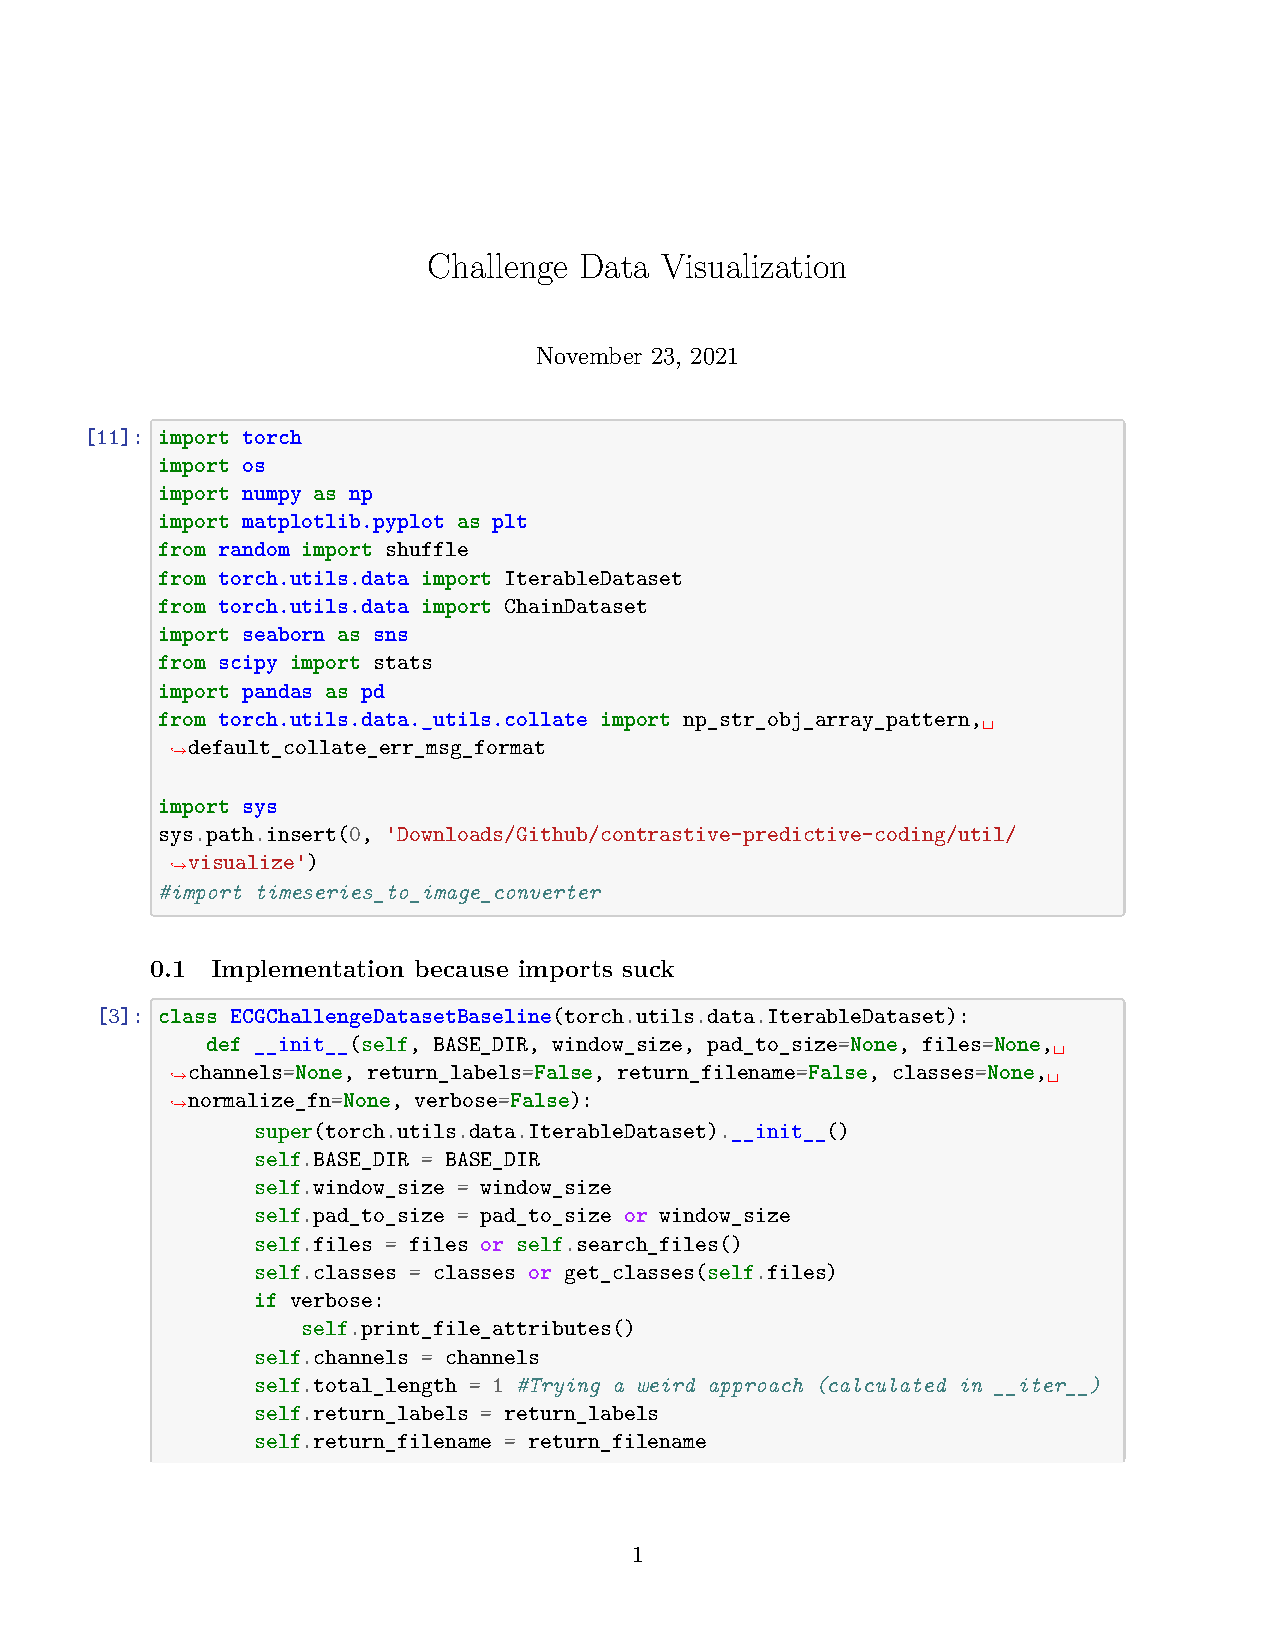
\includepdf[pages=-]{texcode/Challenge Data Visualization.pdf}
%\lstinputlisting[language=Python]{"/home/julian/Downloads/Github/contrastive-predictive-coding/architectures_baseline/baseline_cnn_v0.py"}
